\documentclass[11pt]{article}

\usepackage[a4paper,margin=0.82in]{geometry}
\usepackage[T1]{fontenc}
\usepackage[utf8]{inputenc}
\usepackage{amsmath,amssymb,mathtools}
\usepackage{booktabs,longtable,tabularx,array}
\usepackage{graphicx}
\usepackage{xcolor}
\usepackage{enumitem}
\usepackage{microtype}
\usepackage{hyperref}
\usepackage{float}
\usepackage{caption}
\usepackage{fancyhdr}
\usepackage{url}

\definecolor{navy}{RGB}{26,54,93}
\definecolor{green}{RGB}{47,133,90}
\definecolor{orange}{RGB}{221,107,32}
\definecolor{blue}{RGB}{49,130,206}
\definecolor{lightblue}{RGB}{235,248,255}
\definecolor{lightgreen}{RGB}{240,255,244}
\definecolor{lightorange}{RGB}{255,250,240}
\definecolor{graytext}{RGB}{74,85,104}
\definecolor{lightgray}{RGB}{247,250,252}

\hypersetup{
  colorlinks=true,
  linkcolor=navy,
  urlcolor=blue,
  citecolor=navy,
  pdftitle={From Support Fit to Exact Shared Anatomical Volume Mapping},
  pdfauthor={Abhinay Belde}
}

\graphicspath{{shared_anatomical_volume_report_assets/}}
\setlength{\parindent}{0pt}
\setlength{\parskip}{0.55em}
\setlist[itemize]{leftmargin=1.45em,itemsep=0.25em,topsep=0.25em}
\setlist[enumerate]{leftmargin=1.65em,itemsep=0.25em,topsep=0.25em}
\renewcommand{\arraystretch}{1.18}
\pagestyle{fancy}
\fancyhf{}
\fancyhead[L]{\small Shared Anatomical Footwear Representation}
\fancyhead[R]{\small Technical Progress Report}
\fancyfoot[C]{\thepage}
\setlength{\headheight}{14pt}

\newcommand{\done}{\textcolor{green}{\textbf{Complete}}}
\newcommand{\nextstage}{\textcolor{orange}{\textbf{Next}}}
\newcommand{\notstarted}{\textcolor{graytext}{\textbf{Not started}}}
\newcommand{\R}{\mathbb{R}}

\title{\textbf{From Support Fit to Exact Shared Anatomical Volume Mapping}\\
\large Technical Progress Report Aligned with \texttt{representation.pdf}}
\author{Abhinay Belde}
\date{September 14, 2026}

\begin{document}
\maketitle

\begin{center}
\fcolorbox{green}{lightgreen}{
\begin{minipage}{0.91\linewidth}
\textbf{Current result.} Fifteen accepted normal-shoe instances now have validated,
fold-free tetrahedral volumes connected to one canonical anatomical volume by exact
forward and inverse piecewise-affine maps. All 15 passed independent B3 geometry
validation and Checkpoint 11-C round-trip validation. The semantic anatomical fibers
needed to express the exact coordinate as $(u,v,r)$ remain Checkpoint 11-D.
\end{minipage}}
\end{center}

\vspace{0.5em}
\begin{figure}[H]
  \centering
  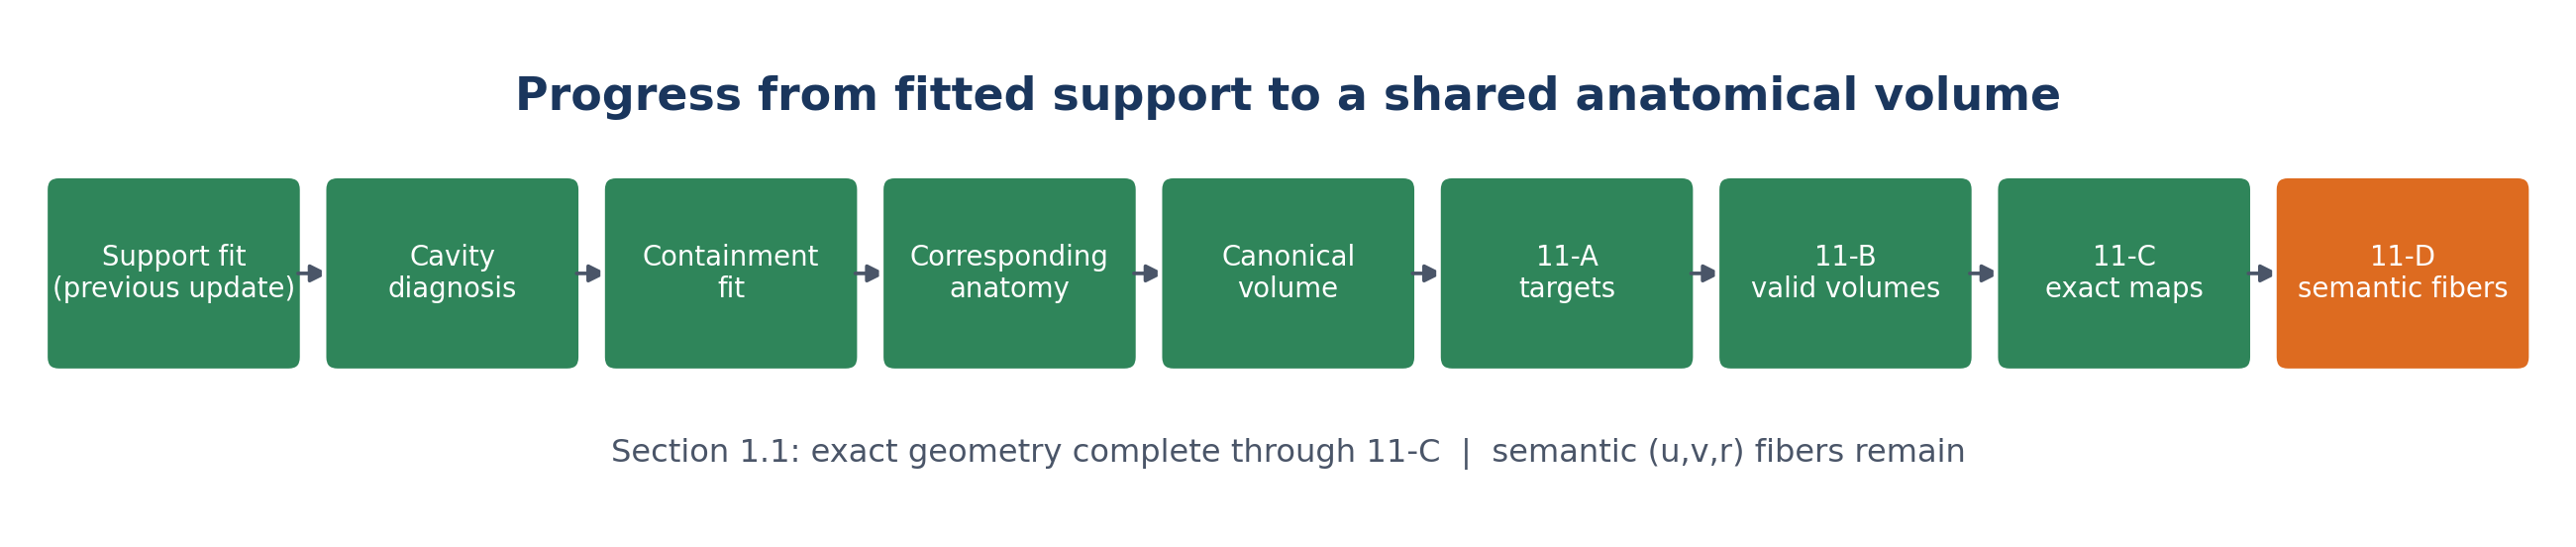
\includegraphics[width=\textwidth]{01_pipeline.png}
  \caption{Implemented pipeline since the previously reported support-fit stage. Green
  stages are complete; orange is the next stage.}
  \label{fig:pipeline}
\end{figure}

\tableofcontents
\newpage

\section{Purpose, scope, and relation to the representation document}

The design document \texttt{notes/representation.pdf} proposes an
\emph{anatomy-grounded volumetric footwear representation}. Its central idea is to
separate a shared anatomical coordinate system from footwear geometry, whose surface
topology may vary arbitrarily. For footwear instance $i$, it defines a fitted foot

\begin{equation}
  F_i = F(\boldsymbol\beta_i,\boldsymbol\theta_i) \subset \R^3,
\end{equation}

a canonical anatomical domain $A$ around a reference foot $F_0$, and a volumetric map

\begin{equation}
  \chi_i:A\rightarrow N(F_i),
  \qquad
  \Phi_i=\chi_i^{-1}.
  \label{eq:document-map}
\end{equation}

The document writes the shared coordinate as

\begin{equation}
  q=\Phi_i(x)=(u,v,r),
\end{equation}

where $(u,v)$ identifies a functional anatomical surface origin and $r$ describes
outward progress through the surrounding volume. It also asks for an approximately
injective, bounded-distortion map instead of a nearest-surface heuristic:

\begin{equation}
  0<c\,\|x_1-x_2\|_2
  \leq \|\Phi_i(x_1)-\Phi_i(x_2)\|_2
  \leq C\,\|x_1-x_2\|_2,
  \qquad C<\infty.
  \label{eq:document-bounded-distortion}
\end{equation}

The implementation reported here realizes this proposal with a canonical tetrahedral
cage, fixed tetrahedron connectivity, a finite-element harmonic $r$ field, bounded
deformation, and exact barycentric lookup. The exact internal coordinate is currently

\begin{equation}
  q_{\mathrm{exact}}=(k,\lambda_0,\lambda_1,\lambda_2,\lambda_3),
  \qquad \sum_{a=0}^{3}\lambda_a=1,
  \label{eq:exact-coordinate}
\end{equation}

where $k$ is a canonical tetrahedron ID. This exact coordinate is implemented and
validated. The remaining 11-D task is to associate it with a semantic surface chart
$(u,v)$ and an anatomical fiber parameterized by $r$.

\subsection{Status at a glance}

\begin{table}[H]
\centering
\small
\begin{tabularx}{\textwidth}{@{}p{0.18\textwidth}X p{0.19\textwidth}p{0.13\textwidth}@{}}
\toprule
\textbf{Implementation stage} & \textbf{Purpose} & \textbf{Document relation} & \textbf{Status}\\
\midrule
Support fit & Seat an articulated SUPR foot on the detected footbed & Prerequisite to Sec.~1.1 & Previously reported\\
Cavity analysis & Measure forbidden collisions and local upper/side clearance & Validates $F_i$ & \done\\
Containment fit & Search anatomical shape, pitch, and placement while preserving support & Constructs fitted $F_i$ & \done\\
Anatomical surface and leg & Transfer stable anatomical identity and extend through the lower leg & Sec.~1.1 boundary construction & \done\\
Canonical volume & Build $A$, its fixed envelope, tetrahedra, and harmonic $r$ & Sec.~1.1 canonical domain & \done\\
11-A & Transfer the computational inner-boundary target to every fitted anatomy & Desired instance boundary & \done\\
11-B & Produce valid instance volumes with fixed topology and no folds & Constructs geometric $\chi_i$ & \done\\
11-C & Implement exact forward/inverse queries and invalid-point classification & Evaluates $\chi_i,\Phi_i$ & \done\\
11-D & Associate volume points with semantic $(u,v,r)$ fibers & Completes semantic Sec.~1.1 coordinate & \nextstage\\
Sec.~1.2 & Learn coverage and material extents in shared coordinates & Structured material field & \notstarted\\
\bottomrule
\end{tabularx}
\caption{Mapping from implementation checkpoints to \texttt{representation.pdf}.}
\end{table}

The initial geometry pipeline produced artifacts for 16 normal-profile shoes. The final
shared-volume scope contains 15 shoes: \texttt{sneaker\_vibe} was deliberately excluded
before B3 because its source shoe geometry has an inconsistent orientation relative to
the accepted normalized set. It was not repaired, loaded, or counted as a B3/11-C
failure.

\section{Starting point: the accepted support fit}

The last reported stage placed a posed SUPR foot on a detected normalized shoe support.
It established plantar seating, heel-to-toe alignment, coordinate transforms, and a
reproducible SUPR shape/pose state. That result answered ``where should the foot sit?'',
but not ``does the complete foot lie in usable shoe space?'' A foot can be well supported
and still cross a sidewall, toe box, upper, or collar. Steps 12 and 13 therefore treated
the accepted support result as immutable input and added explicit cavity reasoning.

Figure~\ref{fig:support-containment} follows \texttt{sandal\_1} through this transition.
This shoe is useful as a running example because its support fit had many detected
collisions, yet its final containment result and later tetrahedral mapping are valid.

\section{Step 12: cavity collision and clearance analysis}
\label{sec:cavity}

\subsection{Geometric objective}

The detected footbed is the only shoe surface on which contact is allowed. Every other
original shoe triangle forms the obstacle surface $\mathcal S_{\mathrm{obs}}$. The ankle
may leave through actual empty opening space, but a real triangle intersection with the
collar remains forbidden. This preserves open sandals and shoe entrances without adding
an artificial lid.

For a foot point $p$, unsigned obstacle clearance is the closest-surface distance

\begin{equation}
  d(p,\mathcal S_{\mathrm{obs}})=
  \min_{y\in\mathcal S_{\mathrm{obs}}}\|p-y\|_2.
\end{equation}

Because the shoe may be open and non-watertight, a global mesh sign is not assumed.
Instead, local signed upper and side clearances are measured by ray intersections with
the corresponding local boundary. When both measurements exist, the conservative
combined clearance is

\begin{equation}
  c(p)=\min\{c_{\mathrm{upper}}(p),c_{\mathrm{side}}(p)\}.
  \label{eq:combined-clearance}
\end{equation}

The same measurement is made at foot vertices and triangle centroids. For face $f$,
with available sample set $S_f$, the conservative face value is

\begin{equation}
  c_f=\min_{s\in S_f}c_s.
\end{equation}

A face is signed outside when $c_f<-\varepsilon$. Exact triangle--triangle tests are
also performed between the foot and obstacle surfaces. If
$\mathcal F_{\mathrm{coll}}$ contains the unique foot faces in exact intersections, the
collision area fraction is

\begin{equation}
  C_{\mathrm{coll}}=
  \frac{\sum_{f\in\mathcal F_{\mathrm{coll}}}A_f}
       {\sum_{f\in\mathcal F_{\mathrm{foot}}}A_f}.
  \label{eq:collision-area}
\end{equation}

Area is used rather than the raw number of intersecting pairs so that a densely
triangulated shoe does not appear artificially worse. Signed protrusion depth and its
area-weighted energy are

\begin{align}
  p_s &= \max(0,-c_s),\\
  e_f &= \frac{1}{|S_f|}\sum_{s\in S_f}p_s^2,\\
  E_{\mathrm{protrusion}} &=
  \frac{\sum_f A_f e_f}{\sum_f A_f}.
  \label{eq:protrusion-energy}
\end{align}

Finally, the affected region is the union of exact collision faces and signed-outside
faces:

\begin{equation}
  \mathcal F_{\mathrm{affected}}
  =\mathcal F_{\mathrm{coll}}\cup\mathcal F_{\mathrm{outside}}.
\end{equation}

Among the final 15-shoe scope, one support fit was already clear and 14 had detected
collisions. A problem status here is a diagnosis, not an execution failure.

\section{Step 13: collision-aware containment fitting}
\label{sec:containment}

\subsection{What was optimized}

The containment search adjusted the actual SUPR anatomical model rather than shrinking
one template uniformly. Its control vector was

\begin{equation}
  \vartheta=
  [\beta_0,\ldots,\beta_9,
  \phi_{\mathrm{ankle}},\phi_{\mathrm{midfoot}},t_x,t_z]^T.
  \label{eq:containment-parameters}
\end{equation}

The ten $\beta$ coefficients change correlated anatomical shape; the two pitch controls
change ankle and midfoot articulation; and $t_x,t_z$ alter heel-to-toe and lateral
placement. Foot size was not a separate free scale. Under the anchored support scale,
length, width, and height changed only through the SUPR shape parameters.

The search enforced fixed, shoe-independent constraints:

\begin{align}
  18\ \mathrm{mm} &\le a(\vartheta)\le 22\ \mathrm{mm},
  &a_{\mathrm{target}}&=20\ \mathrm{mm},\\
  |\Delta\phi_{\mathrm{ankle}}|&\le 4^\circ,
  &|\Delta\phi_{\mathrm{midfoot}}|&\le 4^\circ,\\
  -3&\le \beta_j\le 3.
\end{align}

Every candidate had to return to a valid first contact with the stored support and retain
heel, forefoot, toe, and overall support coverage. It also could not regress beyond the
baseline collision-area tier or baseline signed-outside-area tier.

\subsection{Implemented search mathematics}

This stage did \emph{not} minimize one arbitrary weighted sum of support, collision,
and shape terms. It used a deterministic broad search, local clearance correction, and
lexicographic selection.

The broad search included individual and coupled beta directions and 256 deterministic
Latin-hypercube samples over $\beta_1,\ldots,\beta_9$. For each template, $\beta_0$ was
solved toward 18, 20, and 22 mm toe allowance. Support-valid candidates in the target
band received exact collision tests, and ten beta-diverse candidates were refined.

At a local candidate, near-conflict samples form

\begin{equation}
  \mathcal A=\{j\mid c_j\le h\},
\end{equation}

where $h$ is support-grid spacing. The desired clearance correction is

\begin{equation}
  \Delta c_j^*=\max(0,-c_j+\varepsilon).
\end{equation}

The clearance Jacobian is measured by finite differences of the clearance actually used
in Eq.~\eqref{eq:combined-clearance}:

\begin{equation}
  J_{jk}\approx
  \frac{c_j(\vartheta+\delta_k e_k)-c_j(\vartheta)}{\delta_k}.
\end{equation}

An additional row steers toe position toward the 20 mm target. The joint update is the
minimum-norm least-squares correction

\begin{equation}
  \Delta\vartheta = J^+\Delta c^*,
  \label{eq:containment-update}
\end{equation}

followed by bounds, exact reevaluation, local polling, and line factors
$\{2,1,\tfrac12,\tfrac14\}$. The final exact candidates are ordered by the following
strict priorities:

\begin{equation}
\begin{aligned}
\operatorname{rank}(\vartheta)=(&
\text{toe-band validity},
\text{toe-band distance},
\text{complete containment},\\
&\text{affected-area tier},
\text{collision-area tier},
C_{\mathrm{coll}},
\text{outside-area tier},\\
&\text{maximum protrusion},
E_{\mathrm{protrusion}},
|a-20\ \mathrm{mm}|,
\|\boldsymbol\beta\|_2,\\
&E_{\mathrm{placement}},
E_{\mathrm{support}}).
\end{aligned}
\label{eq:containment-rank}
\end{equation}

Earlier entries dominate later entries; Eq.~\eqref{eq:containment-rank} is not a scalar
sum. The placement-deviation diagnostic is

\begin{equation}
  E_{\mathrm{placement}}=
  \left(\frac{t_x}{h}\right)^2+
  \left(\frac{t_z}{h}\right)^2+
  \left(\frac{\Delta\phi_{\mathrm{ankle}}}{4^\circ}\right)^2+
  \left(\frac{\Delta\phi_{\mathrm{midfoot}}}{4^\circ}\right)^2.
\end{equation}

For \texttt{sandal\_1}, the support-fit baseline had 859 exact intersecting pairs and
$C_{\mathrm{coll}}=0.186662$. The selected containment result had 20.0000066 mm toe
allowance, zero exact collisions, zero signed-outside area, and status
\texttt{contained\_target\_fit}. Across the final 15-shoe scope, five shoes achieved
\texttt{contained\_target\_fit}; ten retained the honest status
\texttt{residual\_target\_fit}. A residual fit is still a plausible authoritative
anatomy. It means that footwear material lying inside that anatomy must later be reported
outside the mathematical footwear-support domain rather than silently mapped.

\begin{figure}[H]
  \centering
  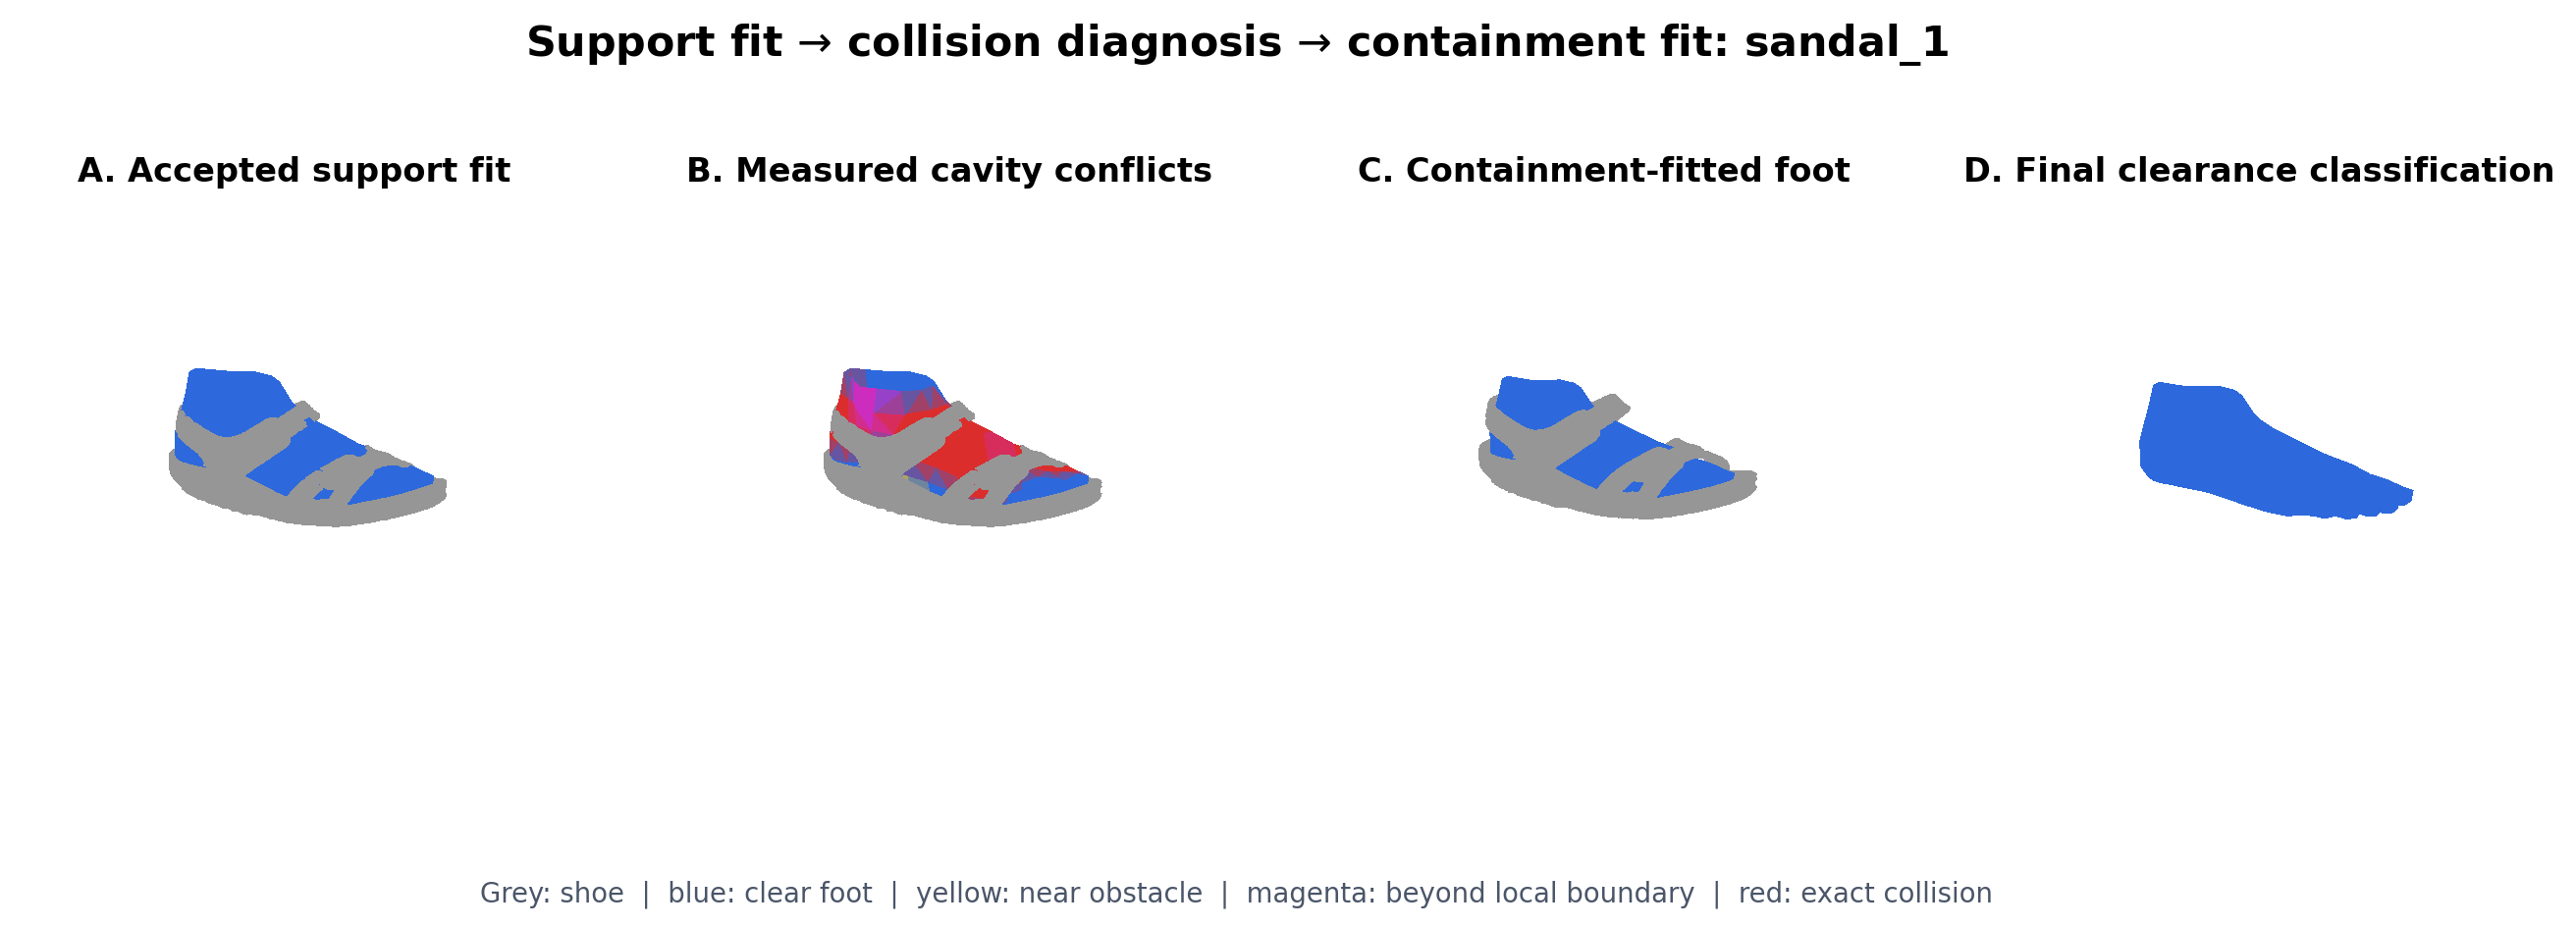
\includegraphics[width=\textwidth]{02_support_cavity_containment.png}
  \caption{Actual saved geometry for \texttt{sandal\_1}. The support fit was valid but
  collided with the sandal. The containment search found a supported, realistic-size
  SUPR foot with no remaining collision for this case.}
  \label{fig:support-containment}
\end{figure}

\section{Steps 14--16: corresponding foot-and-lower-leg anatomy}

The representation requires anatomical meaning to remain stable even though physical
vertex positions change. SUPR supplies stable native vertex and face IDs. A deterministic
two-level subdivision then creates a dense foot containing 4,151 vertices and 8,240
faces; the first 266 vertices remain the accepted native fitted foot exactly.

It is important to separate a \emph{mesh vertex} from a general \emph{surface point}.
The anatomical mesh consists of filled triangles, not only their corner vertices. A
point may therefore lie at a triangle corner, on an edge, or anywhere inside the filled
triangle. Suppose such a point $p_0$ lies on canonical anatomical face
$f_m=(V_{0,a},V_{0,b},V_{0,c})$. Its position can be recorded by the face ID $m$ and
three barycentric weights $\gamma=(\gamma_a,\gamma_b,\gamma_c)$:

\begin{equation}
  p_0=\gamma_a V_{0,a}+\gamma_b V_{0,b}+\gamma_c V_{0,c},
  \qquad \gamma_a+\gamma_b+\gamma_c=1.
\end{equation}

Every fitted SUPR anatomy uses the same anatomical vertex IDs and face IDs. Thus face
$m$ in shoe $i$ has the same anatomical identity but moved corners
$(V_{i,a},V_{i,b},V_{i,c})$. The corresponding surface point is obtained without a new
nearest-point search:

\begin{equation}
  p_i=\gamma_a V_{i,a}+\gamma_b V_{i,b}+\gamma_c V_{i,c}.
  \label{eq:surface-correspondence}
\end{equation}

The face ID and weights stay fixed; only the three corner positions change. Therefore
correspondence means ``the same anatomical address'', not ``the same three-dimensional
position''. This is the basic mechanism later used by Checkpoint 11-A.

The lower-leg stage keeps the dense foot immutable, attaches a near-neutral full-body
SUPR shank at the fitted ankle, and searches limited ankle pitch/roll and tightly bounded
shape correction. Empty entrance space remains allowed; exact contact with actual collar
triangles is measured and retained when natural limits are reached. The joined extended
surface contains 6,951 vertices and 13,832 faces with stable IDs for the foot, ankle
transition, and lower leg. Of the final 15 shoes, 11 had a clear lower-leg exit and four
retained residual collar intersections.

\begin{figure}[H]
  \centering
  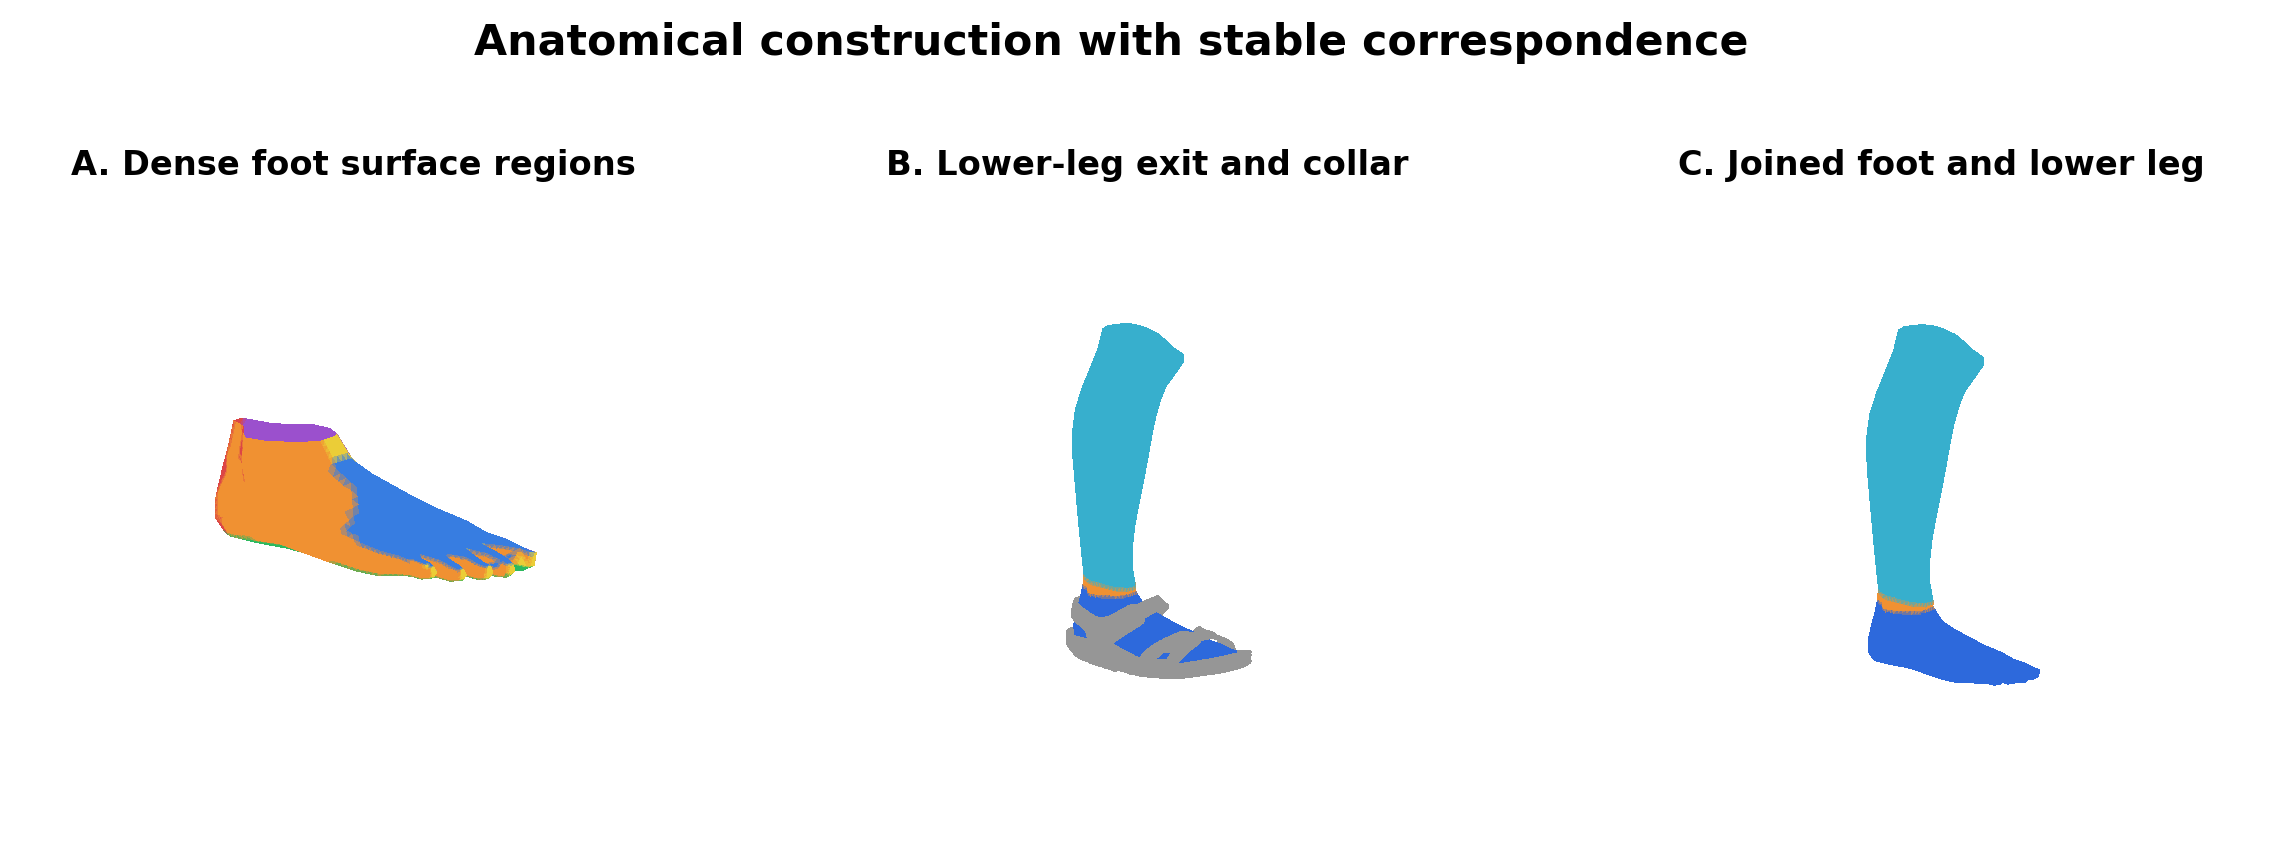
\includegraphics[width=\textwidth]{03_corresponding_anatomy.png}
  \caption{Actual anatomical outputs for \texttt{sandal\_1}. Region colors remain tied
  to the same anatomy while the lower leg and ankle transition extend the domain for
  boots and shoe collars.}
  \label{fig:anatomy}
\end{figure}

\section{Step 17: canonical tetrahedral anatomical volume}
\label{sec:canonical-volume}

\subsection{Authoritative anatomy versus computational boundary}

The 6,951-vertex fitted surface is authoritative and is never repaired in place. The
canonical neutral foot contains native toe self-overlap, which is unsuitable as a closed
tetrahedral boundary. A separate computational copy is therefore repaired, subdivided,
reattached to the unchanged dense lower leg, and closed at the knee. Two-way surface
face-and-barycentric maps preserve its connection to the authoritative anatomy.

These are two different meshes with two different jobs:

\begin{itemize}
  \item The \textbf{authoritative anatomical surface} preserves the original anatomical
  meaning and SUPR correspondence. Its extended foot-and-lower-leg version has 6,951
  vertices and 13,832 faces.
  \item The \textbf{computational boundary} is the clean, closed surface used to build
  the tetrahedral volume. It has been repaired near problematic toes and includes a
  computational knee cap. It is not a replacement for the authoritative anatomy.
\end{itemize}

Because the meshes have different vertices and faces, a computational vertex is not
assumed to equal an anatomical vertex. Instead, each computational vertex is attached
to a precisely recorded point on the authoritative surface. This attachment is explained
step by step in Section~\ref{sec:11a}.

This produces a computational inner boundary with 8,224 vertices and 16,444 faces. A
fixed outer envelope has 642 vertices and 1,280 faces. Gmsh fills the shell with 14,440
volume vertices and 59,081 positively oriented first-order tetrahedra while preserving
the supplied boundary vertices and triangles.

The outer surface is a fourth-order superellipsoid:

\begin{equation}
  \sum_{d\in\{x,y,z\}}
  \left|\frac{x_d-c_d}{a_d}\right|^4=1,
  \qquad
  c=(0.45,-0.825,0),
  \quad a=(0.85,1.225,0.48).
  \label{eq:envelope}
\end{equation}

The same envelope is kept bitwise fixed for every shoe. Consequently the shoe geometry
does not redefine the coordinate system.

\subsection{Finite-element harmonic outward coordinate}

The canonical scalar $r$ minimizes Dirichlet energy

\begin{equation}
  E_r(r)=\frac12\int_A\|\nabla r\|_2^2\,dV,
\end{equation}

equivalently satisfying

\begin{equation}
  \nabla^2 r=0\quad\text{in }A,
  \qquad
  r=0\ \text{on anatomical skin},
  \qquad
  r=1\ \text{on the outer envelope}.
  \label{eq:harmonic-r}
\end{equation}

The computational knee cap is a closure, not anatomy; its non-rim vertices receive the
natural boundary condition rather than fixed $r=0$. For linear tetrahedral basis
functions $N_a$, the local stiffness matrix is

\begin{equation}
  K_{ab}^{(k)}=V_k\,\nabla N_a\cdot\nabla N_b,
\end{equation}

and after assembling the global matrix, the free values solve

\begin{equation}
  K_{II}r_I=-K_{IB}r_B.
  \label{eq:harmonic-linear-system}
\end{equation}

This $r$ is a normalized harmonic layer coordinate, not physical distance in
millimetres. It is stored canonically and later transported with exact tetrahedral
coordinates.

\begin{figure}[H]
  \centering
  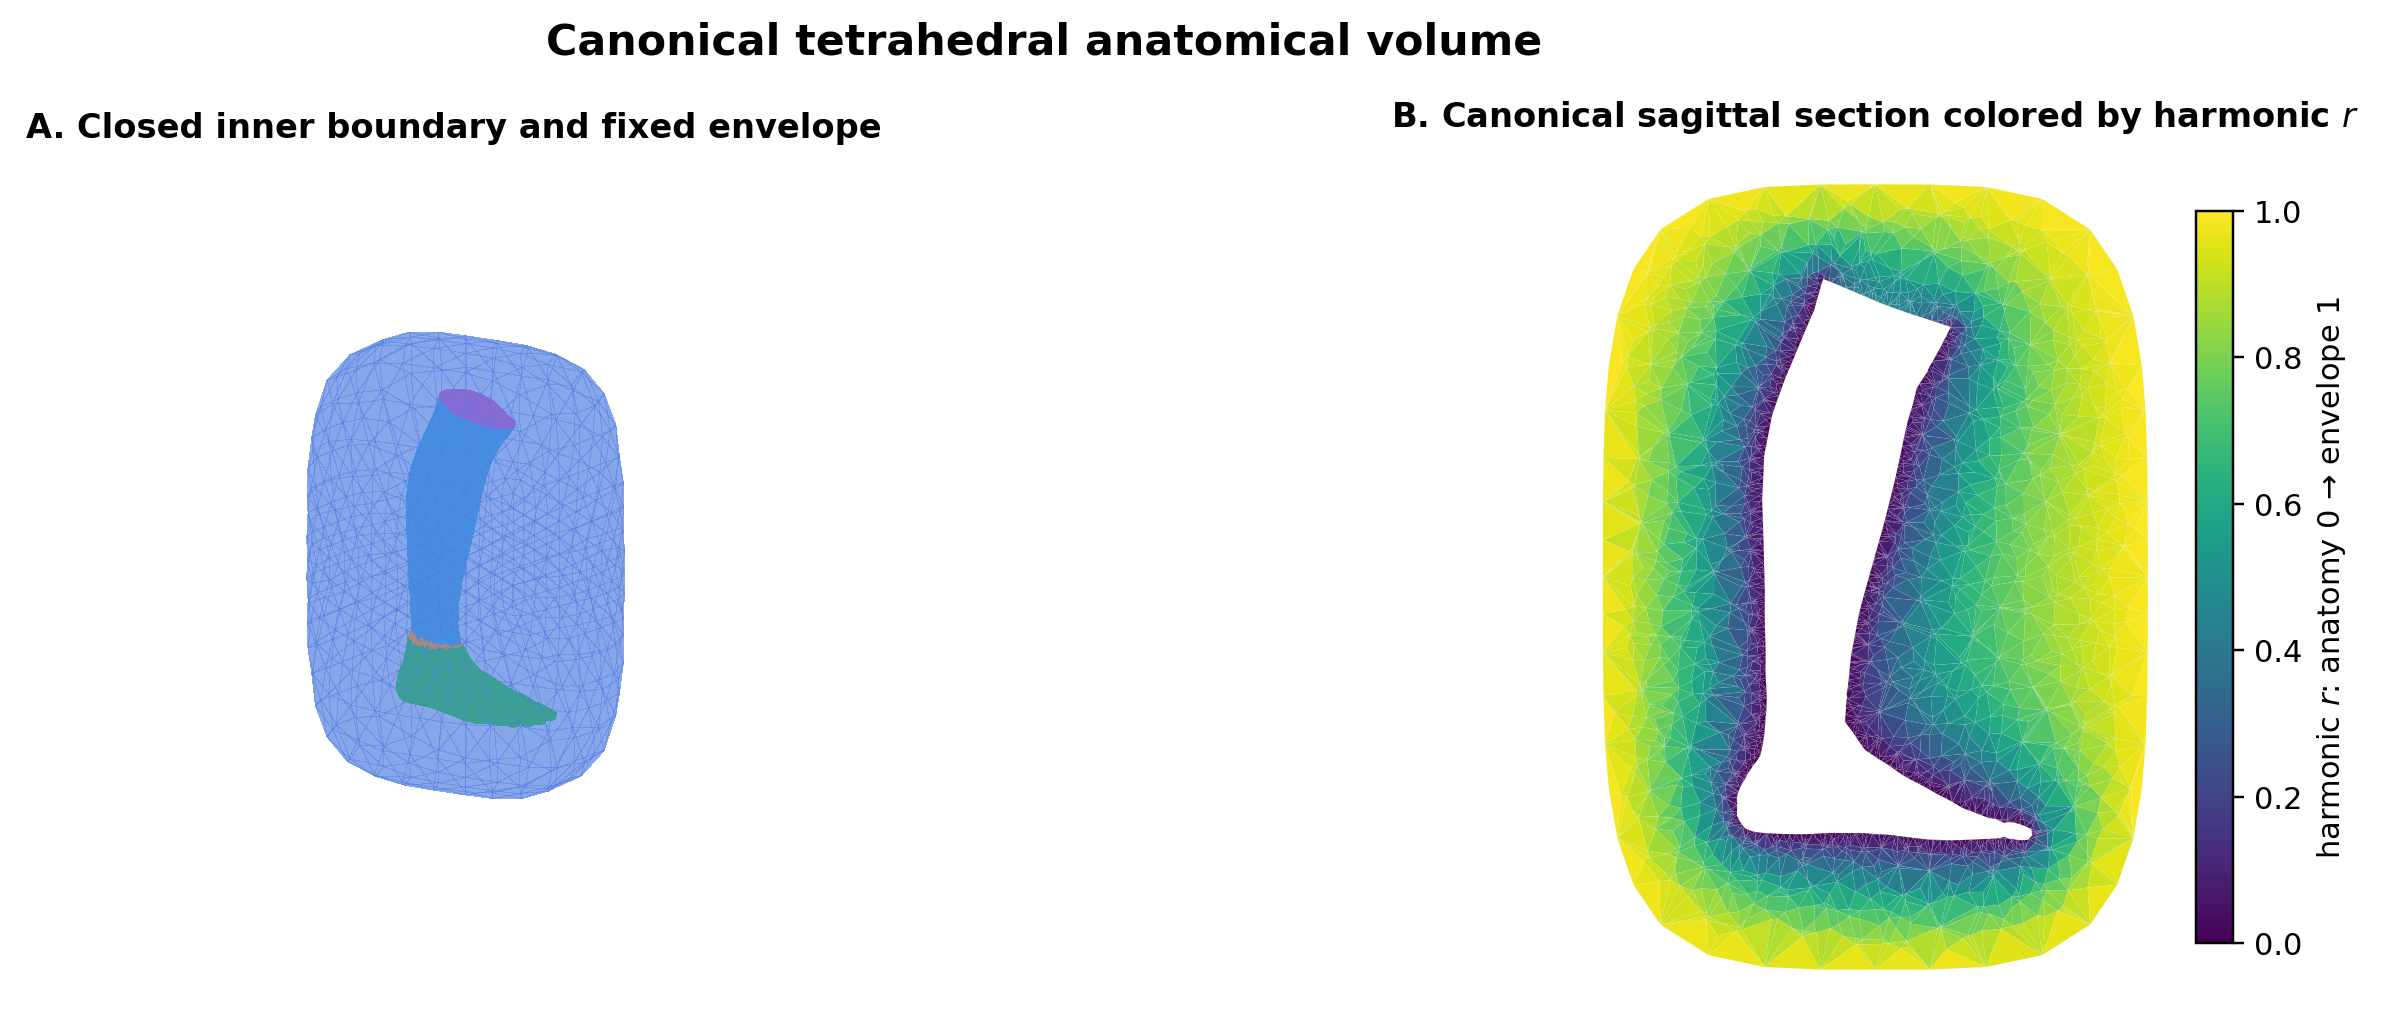
\includegraphics[width=\textwidth]{04_canonical_volume.png}
  \caption{Canonical domain $A$. Left: labeled inner boundary inside the translucent
  fixed envelope. Right: an actual sagittal tetrahedral section colored by the solved
  harmonic $r$ field.}
  \label{fig:canonical-volume}
\end{figure}

\section{Checkpoint 11-A: fitted computational-boundary targets}
\label{sec:11a}

\subsection{Notation used in the construction}

The following symbols distinguish the anatomical mesh, the computational mesh, and a
shoe-specific target. The two subscripts have simple meanings: $i$ identifies the shoe,
whereas $j$ identifies a computational-boundary vertex.

\begin{table}[H]
\centering
\small
\begin{tabularx}{\textwidth}{@{}p{0.20\textwidth}X@{}}
\toprule
\textbf{Symbol} & \textbf{Meaning}\\
\midrule
$i$ & Shoe or fitted-foot instance index, for example \texttt{sandal\_1}.\\
$j$ & Vertex index on the computational inner boundary, $j=1,\ldots,8224$.\\
$a,b,c$ & Three authoritative anatomical vertex indices forming one anatomical face.\\
$m$ & ID of an authoritative anatomical triangular face.\\
$V_{0,a}$ & Position of anatomical vertex $a$ on the neutral canonical reference anatomy.\\
$V_{i,a}$ & Position of that same anatomical vertex $a$ after fitting the anatomy to shoe $i$.\\
$C_j$ & Position of computational-boundary vertex $j$ in the canonical reference.\\
$P_j$ & Closest point on the canonical authoritative anatomical surface to $C_j$; it is
not a newly inserted vertex and is not random.\\
$\gamma_j$ & Three barycentric weights recording where $P_j$ lies in its anatomical face.\\
$T_{i,j}$ & Desired position of computational vertex $j$ on the fitted anatomy for shoe $i$;
this is the 11-A target vertex.\\
\bottomrule
\end{tabularx}
\caption{Variables used to construct a Checkpoint 11-A target.}
\label{tab:11a-notation}
\end{table}

\subsection{Step 1: attach the canonical computational mesh to the canonical anatomy}

Consider one canonical computational vertex $C_j$. It lies near the canonical
authoritative anatomy, but it generally does not coincide with one of its 6,951 vertices
because the two meshes have different topology and resolution. We search the complete
filled triangular anatomical surface for the closest point:

\begin{equation}
  P_j=\operatorname*{arg\,min}_{p\in S_0^{\mathrm{anat}}}
      \|C_j-p\|_2,
  \label{eq:11a-closest-point}
\end{equation}

where $S_0^{\mathrm{anat}}$ is the canonical authoritative anatomical surface. ``A point
on the surface'' means any location inside any filled triangle, including its edges and
corners; it does not mean only an existing mesh vertex.

Suppose the resulting point $P_j$ lies on anatomical face
$f_m=(V_{0,a},V_{0,b},V_{0,c})$. We calculate weights satisfying

\begin{equation}
  P_j=\gamma_{j,a}V_{0,a}
      +\gamma_{j,b}V_{0,b}
      +\gamma_{j,c}V_{0,c},
  \qquad
  \gamma_{j,a}+\gamma_{j,b}+\gamma_{j,c}=1.
  \label{eq:11a-reference-attachment}
\end{equation}

For vertex $C_j$, we save the face ID $m$ and these three weights. Together they form an
exact anatomical address for $P_j$. Multiple computational vertices may attach to
different points in the same anatomical triangle; they then share the face ID but have
different weights.

\subsection{Step 2: evaluate the same anatomical address on fitted shoe $i$}

The fitted foot is the desired anatomy for shoe $i$. It has the same authoritative
vertex IDs and face IDs as the canonical anatomy, although its vertices have moved due
to shape, pose, and placement. Therefore, the canonical face
$(V_{0,a},V_{0,b},V_{0,c})$ corresponds directly to fitted face
$(V_{i,a},V_{i,b},V_{i,c})$.

Checkpoint 11-A reuses the stored face ID and the same weights on that fitted face:

\begin{equation}
  T_{i,j}=\gamma_{j,a}V_{i,a}
          +\gamma_{j,b}V_{i,b}
          +\gamma_{j,c}V_{i,c}.
  \label{eq:11a-target}
\end{equation}

Thus $T_{i,j}$ means: ``where computational vertex $j$ should be placed to represent
the same anatomical location on fitted shoe $i$.'' No closest-point search is repeated
on the fitted foot. Repeating that search could allow the attachment to jump to a nearby
but anatomically different toe. Reusing the face ID and weights preserves identity.

This operation is repeated for all 8,224 computational vertices:

\begin{equation}
  \underbrace{C_j}_{\text{canonical computational vertex}}
  \longrightarrow
  \underbrace{(m,\gamma_j)}_{\text{saved anatomical address}}
  \longrightarrow
  \underbrace{T_{i,j}}_{\text{target on fitted anatomy}}.
  \label{eq:11a-story}
\end{equation}

The collection $T_i=\{T_{i,1},\ldots,T_{i,8224}\}$ is a new target mesh. Its vertex
positions follow fitted anatomy $i$, while its faces, vertex numbering, and connectivity
remain those of the canonical computational boundary. The actual fitted anatomical
surface is neither replaced nor edited.

\subsection{What 11-A has and has not accomplished}

At this point the desired inner boundary is known, so tetrahedral movement can begin in
Checkpoint 11-B. However, 11-A has moved only the target surface positions. It has not
yet moved the surrounding tetrahedral interior, fixed the outer envelope, or guaranteed
that the target surface is geometrically valid.

A clean reference proxy is not guaranteed to remain intersection-free after
Eq.~\eqref{eq:11a-target}. Moving a fixed triangle network onto a narrower or differently
articulated toe configuration can make non-neighboring triangles cross. Therefore 11-A
is a \emph{corresponding desired boundary}, not a cleaned final mesh. Within the final
15-shoe scope, six targets were directly \texttt{ready}; nine were
\texttt{ready\_requires\_untangling}. Only foot-skin intersections were allowed at this
stage; bridge, lower-leg, or knee-cap intersections would fail validation.

\begin{figure}[H]
  \centering
  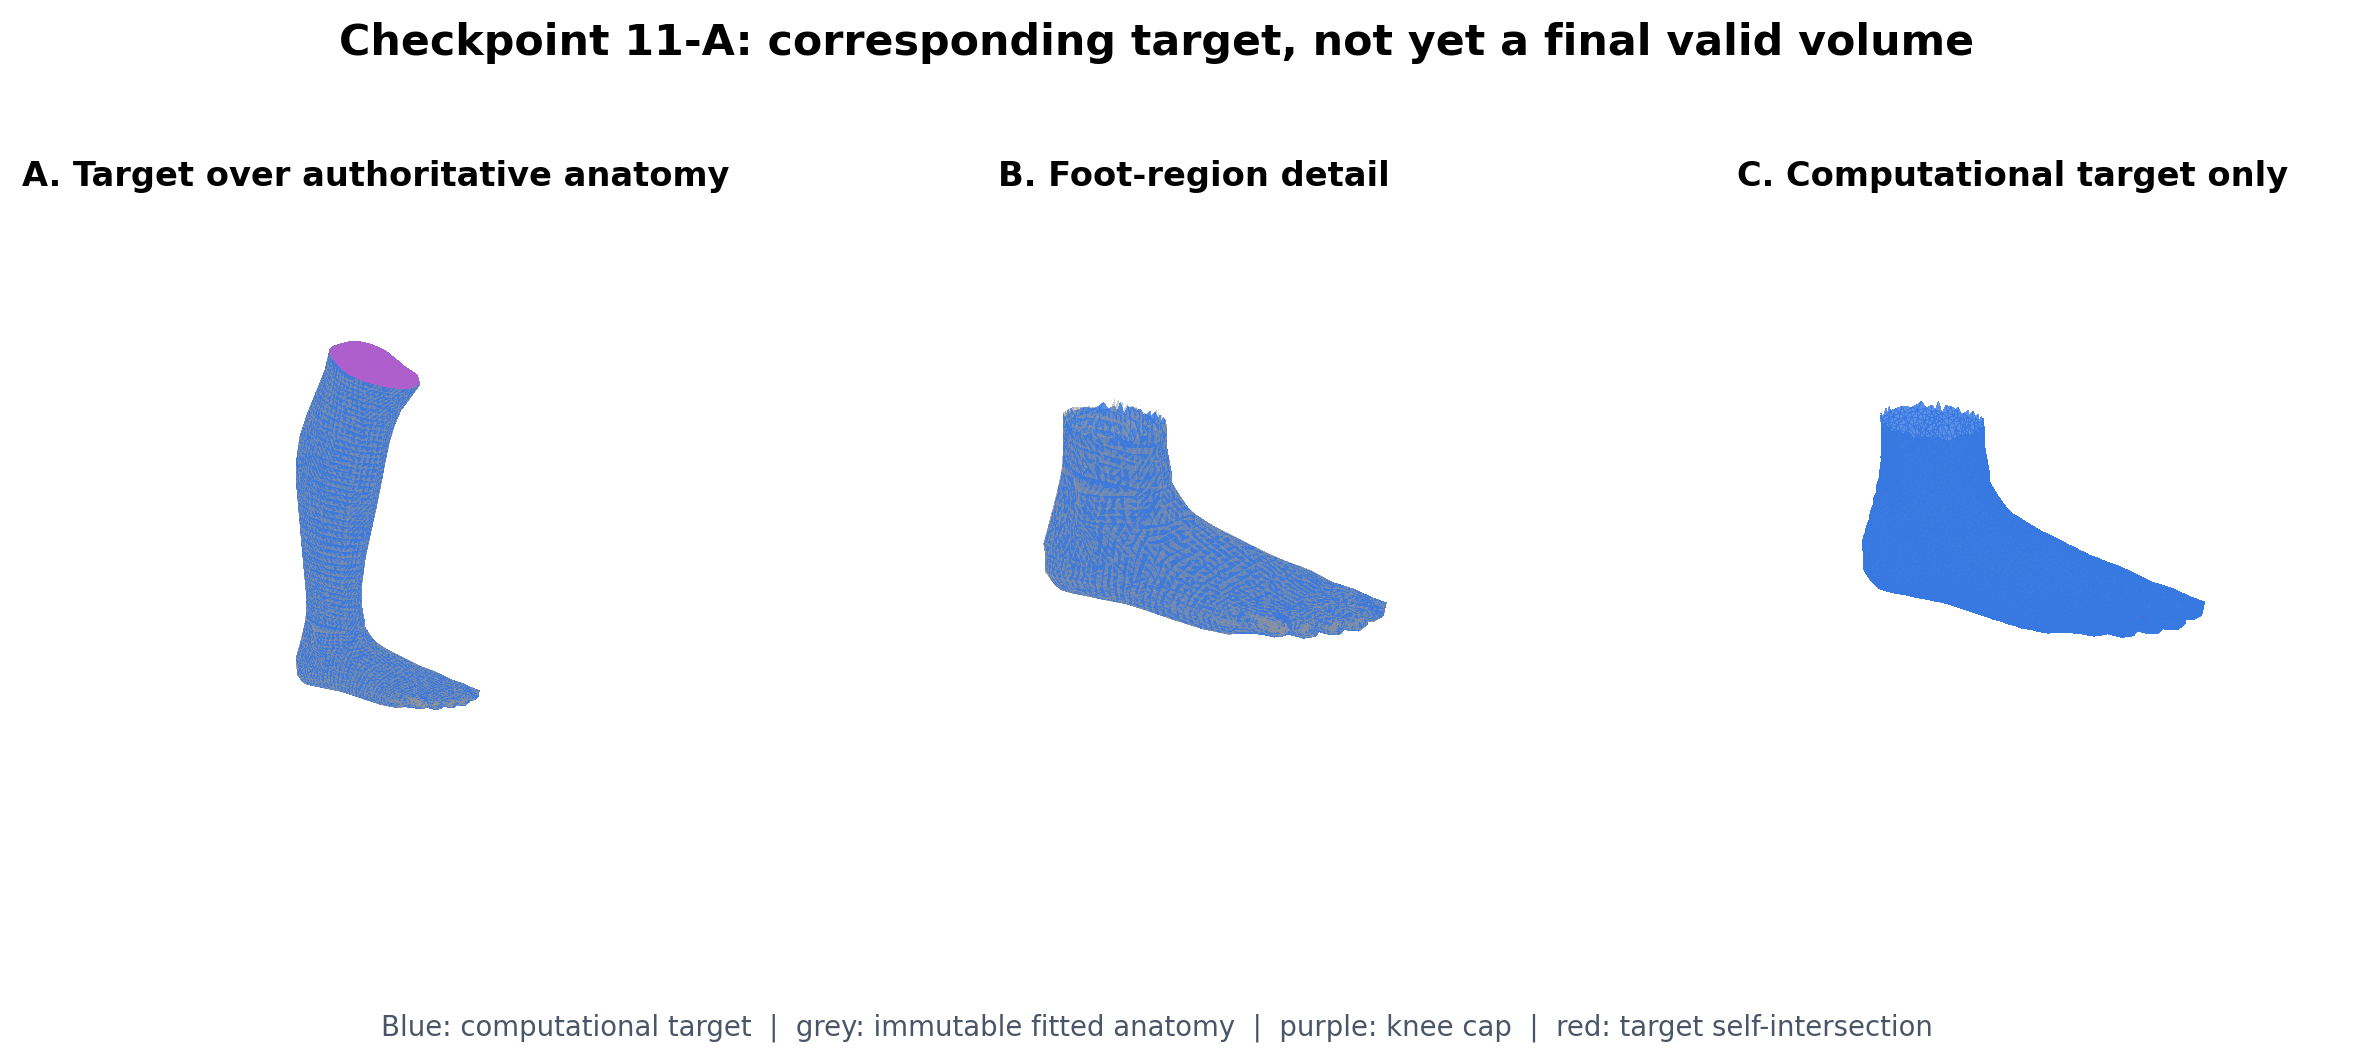
\includegraphics[width=\textwidth]{05_boundary_target.png}
  \caption{Checkpoint 11-A for \texttt{sandal\_1}. The overlay validates anatomical
  proximity and correspondence. Red triangles mark target self-intersections that the
  later B3 computational-surface repair must resolve.}
  \label{fig:11a}
\end{figure}

\section{Checkpoint 11-B: valid shoe-specific volume deformation}
\label{sec:11b}

Checkpoint 11-A tells us where each of the 8,224 inner-boundary vertices \emph{wants} to
go, but it does not move the tetrahedra around the foot. Checkpoint 11-B performs that
movement.

One can picture the canonical volume as flexible foam between two surfaces. Its inner
surface is the computational foot, its outer surface is the fixed envelope, and its
interior is divided into 59,081 numbered tetrahedra. For shoe $i$, 11-B moves the inner
surface toward the target $T_i$, keeps the outer surface fixed, and moves the intervening
vertices smoothly. The tetrahedron numbers and connections never change. Therefore,
tetrahedron $k$ retains the same canonical identity even though its physical corner
positions change for each shoe.

The movement cannot be performed by simply replacing every $C_j$ with $T_{i,j}$. Doing
so would move only the skin and could flatten, invert, or overlap the tetrahedra attached
to it. The boundary and interior must be moved together while checking that the volume
remains a valid one-to-one domain.

\subsection{Notation used in the deformation}

\begin{table}[H]
\centering
\small
\begin{tabularx}{\textwidth}{@{}p{0.20\textwidth}X@{}}
\toprule
\textbf{Symbol} & \textbf{Meaning}\\
\midrule
$Q$ & All canonical volume-vertex positions before deformation. On the inner boundary,
these positions include the computational vertices $C_j$.\\
$T_i$ & Complete 11-A inner-boundary target for shoe $i$; its $j$th position is $T_{i,j}$.\\
$U$ & Displacement of volume vertices from their canonical positions.\\
$X$ & Current or final positions of all volume vertices during deformation.\\
$I$ and $B$ & Interior/free volume vertices and prescribed boundary vertices,
respectively.\\
$K$ & Finite-element stiffness matrix that couples neighboring volume vertices and
produces a smooth displacement.\\
$\alpha$ & B2 progress from the canonical volume ($0$) toward the complete smooth target
deformation ($1$).\\
$\beta$ & B3 progress from the canonical inner surface ($0$) toward the complete 11-A
target ($1$).\\
$k$ & Canonical tetrahedron ID.\\
$F_k$ & Local deformation matrix of tetrahedron $k$ from canonical to current shape.\\
$J_k=\det(F_k)$ & Local signed volume ratio. A positive value preserves orientation;
zero is flat; a negative value is inside-out.\\
$\sigma_{\min},\sigma_{\max}$ & Smallest and largest local stretch factors of $F_k$.\\
$\kappa$ & Condition number $\sigma_{\max}/\sigma_{\min}$, measuring anisotropic
distortion.\\
$h$ & One fixed characteristic spacing of the fitted surface, used to normalize lengths.\\
\bottomrule
\end{tabularx}
\caption{Main variables used by Checkpoint 11-B.}
\label{tab:11b-notation}
\end{table}

The required result has a fixed outer envelope, positive cell orientation, bounded
distortion, no inner self-intersection, no inner--outer intersection, and only a bounded
deviation from the authoritative fitted anatomy.

\subsection{B1: strict input validation}

B1 cross-validates the canonical volume, 11-A target, and authoritative fitted anatomy:
schema and stage names, shoe identity, profile, array dimensions, finite values,
topology and geometry digests, correspondence arrays, surface fidelity, recorded
intersection pairs, and frozen-envelope containment. In simple terms, B1 confirms that
the canonical foam, desired inner surface, and fitted anatomy belong together and have
not been silently changed. It is a diagnostic gate and performs no deformation.

\subsection{B2: smooth finite-element continuation}

For inner-boundary vertex $j$, the required displacement is the arrow from its canonical
position $C_j$ to its 11-A target $T_{i,j}$. Collecting those arrows for the complete
boundary gives

\begin{equation}
  U_{\partial,\mathrm{inner}}=T_i-Q_{\partial,\mathrm{inner}},
  \qquad
  U_{\partial,\mathrm{outer}}=0.
\end{equation}

Here $Q_{\partial,\mathrm{inner}}$ is the collection of canonical computational-boundary
positions, so its $j$th entry is $C_j$. The second equation says that every outer-envelope
vertex has exactly zero displacement.

The unknown displacements of the interior vertices are then chosen to vary smoothly
between the moving inner surface and the stationary outer surface. The same tetrahedral
stiffness matrix used for harmonic $r$ gives

\begin{equation}
  K_{II}U_I=-K_{IB}U_B.
  \label{eq:b2-fem}
\end{equation}

$U_B$ contains the already prescribed inner and outer boundary movements, and $U_I$
contains the unknown interior movements. $K_{II}$ describes how free interior vertices
are connected to one another, while $K_{IB}$ describes how they are connected to the
boundary. Solving the equation makes the interior follow the boundary smoothly.

Because this baseline is linear, continuation evaluates

\begin{equation}
  X(\alpha)=Q+\alpha U,
  \qquad 0\le\alpha\le1.
  \label{eq:b2-continuation}
\end{equation}

At $\alpha=0$, $X(0)=Q$, so nothing has moved. At $\alpha=1$, B2 has attempted the
complete smooth movement. Intermediate values move every vertex by the same fraction of
its computed displacement.

Trials begin with a step of 0.25. A failed trial is discarded and the step is halved
until the $10^{-4}$ minimum. For tetrahedron $k$, B2 monitors the orientation ratio

\begin{equation}
  J_k(\alpha)=
  \frac{V_k(X(\alpha))}{V_k(Q)}.
\end{equation}

The ratio $J_k=1$ means that cell $k$ retains its canonical signed volume, a small
positive value means that it has become nearly flat, and a non-positive value means that
it is flat or inside-out. B2 rejects non-finite vertices, $J_k<10^{-6}$, degenerate
inner faces, envelope escape, inner self-intersections, and inner--outer intersections.
If a trial fails, B2 returns to the preceding valid state and tries a smaller progress
step. Its last valid state is only a safe starting point, not necessarily the final
answer. For \texttt{sandal\_1}, B2 stopped safely at $\alpha=0.769043$ rather than
flattening or inverting the limiting cells.

\subsection{B3: localized bounded-distortion optimization}

B2 may stop because an exact 11-A target would make a few toe triangles cross or a few
attached tetrahedra become too flat. B3 resolves this by allowing small corrections to
the \emph{computational copy only}. The authoritative fitted anatomy and saved 11-A
target are never edited.

B3 starts with the local surface region containing the 11-A intersection faces and weak
boundary tetrahedra. Vertices outside that region follow the current target exactly. The
initial region is expanded by two neighboring face rings and may grow deterministically;
a full-surface fallback exists if a local region is insufficient. The optimizer then
advances the desired boundary toward $\beta=1$, while keeping each permitted correction
within $0.5h$. Once the corrected surface reaches complete target progress, it is fixed
and the tetrahedral interior is solved between that surface and the unchanged outer
envelope.

The target continuation is

\begin{equation}
  T_i(\beta)=(1-\beta)Q_{\partial,\mathrm{inner}}+\beta T_i,
  \qquad 0\le\beta\le1.
\end{equation}

Thus $T_i(0)$ is the canonical inner boundary and $T_i(1)=T_i$ is the complete 11-A
target. The parameter $\beta$ lets B3 solve a sequence of smaller, safer problems rather
than demanding the full difficult shape in one jump.

For a canonical tetrahedron and its deformed instance,

\begin{align}
  D_k^0 &= [Q_1-Q_0\quad Q_2-Q_0\quad Q_3-Q_0],\\
  D_k   &= [X_1-X_0\quad X_2-X_0\quad X_3-X_0],\\
  F_k   &= D_k(D_k^0)^{-1},
  &J_k&=\det(F_k).
  \label{eq:deformation-gradient}
\end{align}

The implemented normalized objective is

\begin{equation}
  E=10E_{\mathrm{target}}+E_{\mathrm{surface}}+E_{\mathrm{FEM}}
    +0.1E_{\mathrm{distortion}}+E_{\mathrm{barriers}}.
  \label{eq:b3-total}
\end{equation}

For active inner vertices $\mathcal I$, global surface area weights $w_j$, all
computational-boundary edges $\mathcal E$, and surface resolution $h$,

\begin{align}
E_{\mathrm{target}}
  &=\sum_{j\in\mathcal I}w_j
    \left\|\frac{X_j-T_{i,j}(\beta)}{h}\right\|_2^2,\\
E_{\mathrm{surface}}
  &=\frac{1}{|\mathcal E|}
    \sum_{(a,b)\in\mathcal E_{\mathrm{incident}}}
    \left\|
    \frac{(X_b-X_a)-(T_{i,b}(\beta)-T_{i,a}(\beta))}{h}
    \right\|_2^2,\\
E_{\mathrm{FEM}}
  &=\frac{(X-B(\beta))^T K(X-B(\beta))}{V_A},\\
E_{\mathrm{distortion}}
  &=\sum_k \widehat V_k\left[
    \frac{\|F_k\|_F^2}{3J_k^{2/3}}-1+0.1(\log J_k)^2
    \right].
  \label{eq:b3-components}
\end{align}

Here $B(\beta)$ is the smooth FEM baseline, $V_A$ is canonical shell volume, and
$\widehat V_k$ are normalized canonical cell-volume weights. The distortion expression
is scale-aware AMIPS with explicit volume control.

The determinant, collision-gap, envelope, and correction-cap barriers share a smooth
one-sided form. For a lower-bounded value $x>f$ activated below $a$, let
$y=(x-f)/(a-f)$. Then

\begin{equation}
  b_{\mathrm{lower}}(x)=
  \begin{cases}
  -(1-y)^2\log y, & f<x<a,\\
  0, & x\ge a,\\
  +\infty, & x\le f.
  \end{cases}
  \label{eq:barrier}
\end{equation}

The determinant barrier activates below 0.1 and has emergency floor $10^{-6}$.
Collision protection activates below $0.25h$ and keeps a numerical separation above
$10^{-4}h$. Computational-boundary correction is capped at $0.5h$. Barrier multipliers
increase through $1,10,100,100$. Analytical gradients are supplied to deterministic
CPU L-BFGS-B; exact triangle intersection tests, rather than the approximate barrier,
remain the acceptance authority.

Final acceptance requires

\begin{equation}
\begin{gathered}
  \beta=1,\qquad \min_k J_k\ge0.02,\qquad
  \min_k\sigma_{\min}(F_k)\ge0.05,\\
  \max_k\sigma_{\max}(F_k)\le5,qquad
  \max_k\kappa(F_k)\le20,\\
  \text{zero inner self-intersections},\qquad
  \text{zero inner--outer intersections},\\
  \max_j\|X_j-T_{i,j}\|\le0.5h,qquad
  0.5\le A_f(X)/A_f(T_i)\le2.0,
\end{gathered}
\label{eq:b3-acceptance}
\end{equation}

plus exact outer-envelope equality and region-specific reverse fidelity to the immutable
fitted anatomy.

\begin{figure}[H]
  \centering
  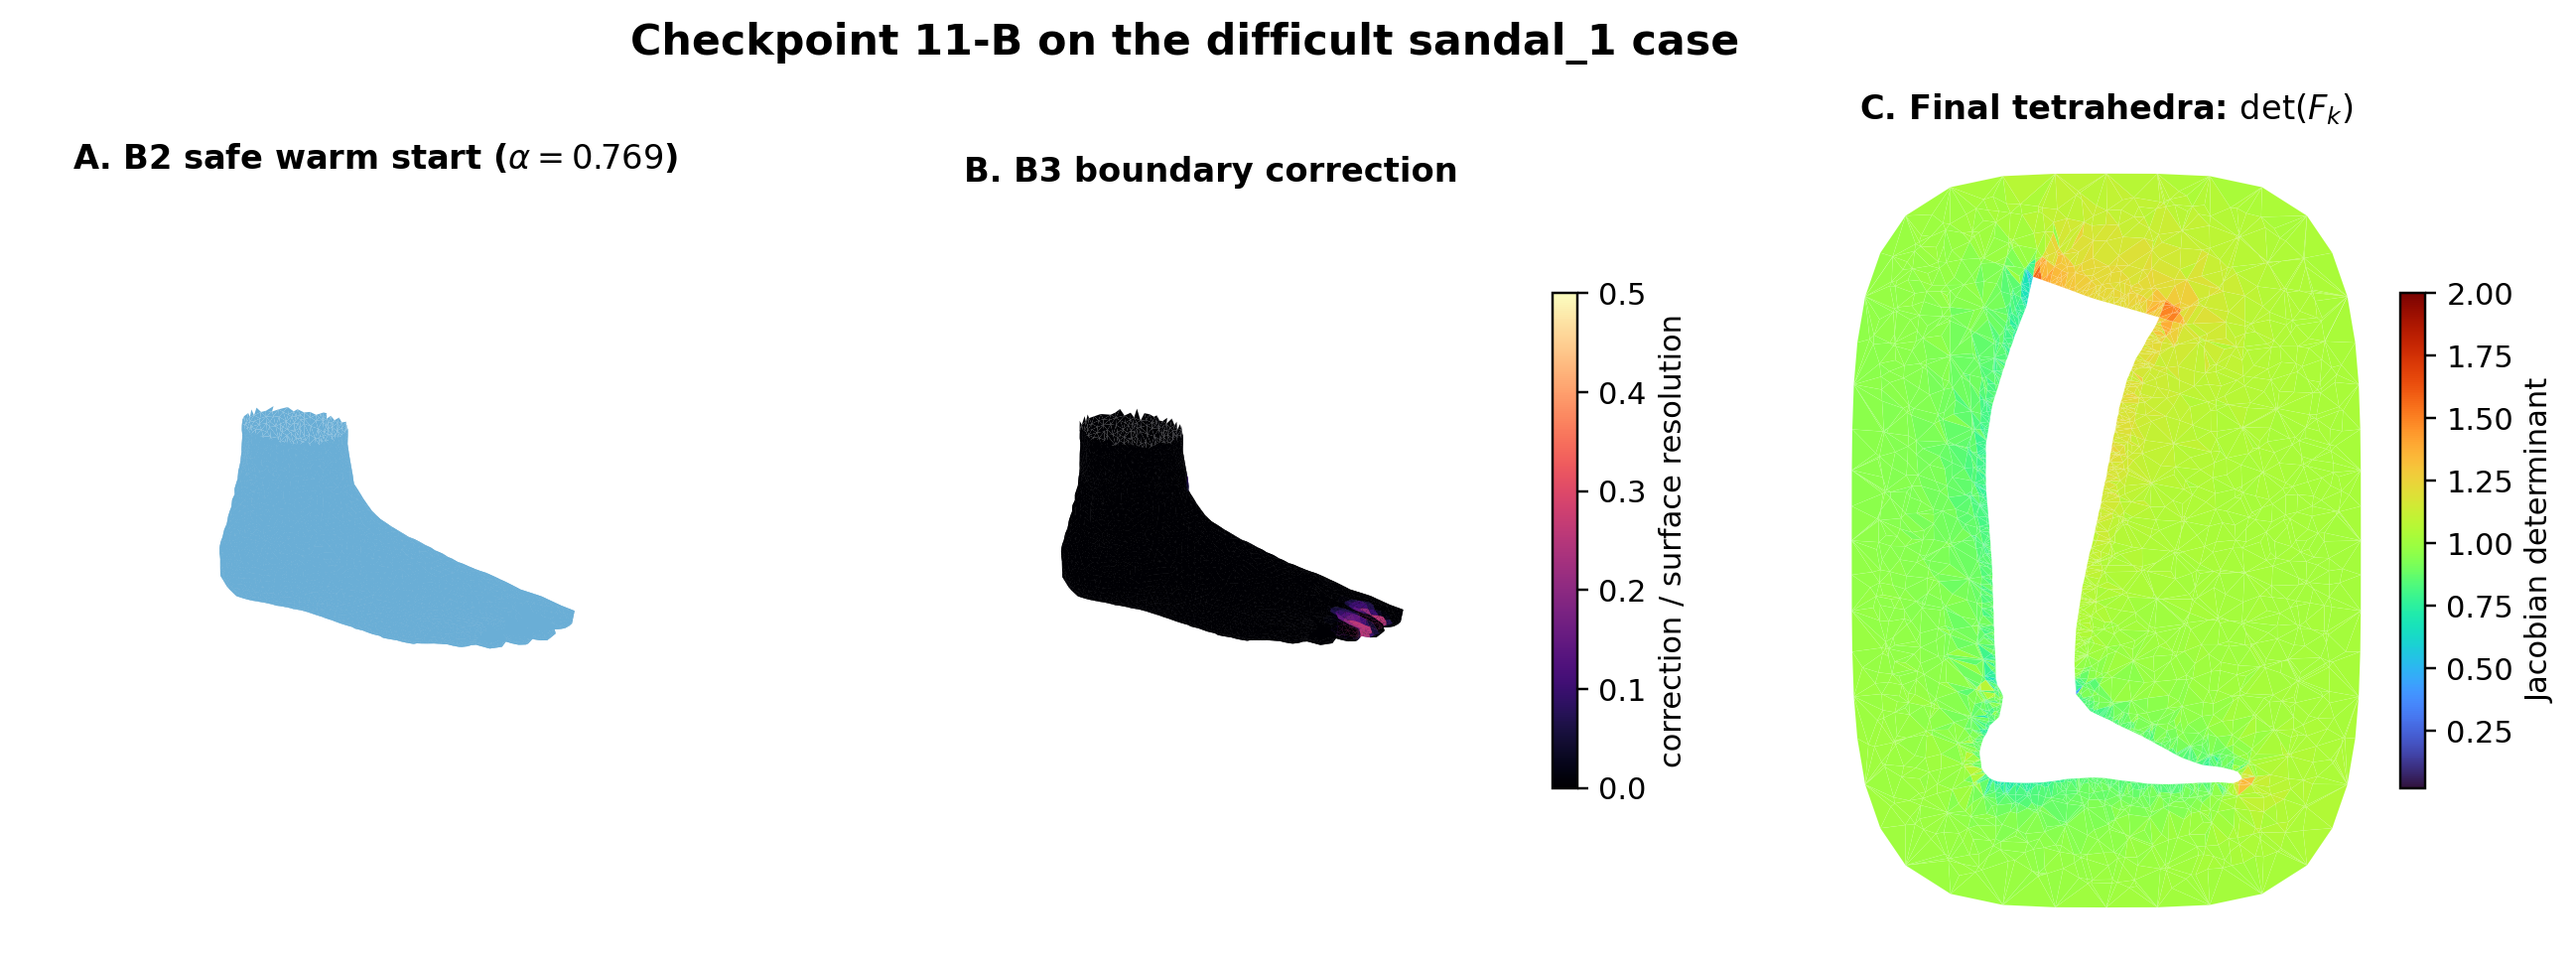
\includegraphics[width=\textwidth]{06_b3_deformation.png}
  \caption{B2 and B3 on \texttt{sandal\_1}. B2 preserves the last safe state. B3 uses
  small, localized computational-boundary corrections and produces a positive,
  bounded-distortion final tetrahedral volume.}
  \label{fig:b3}
\end{figure}

\subsection{Final 15-shoe result}

All 15 accepted shoes reached $\beta=1$ and passed independent post-run geometric
revalidation. Four are \texttt{final\_exact\_target}; 11 are
\texttt{final\_corrected\_target}; none failed. Every final mesh has zero inner
self-intersections, zero inner--outer intersections, and an outer envelope bitwise equal
to the canonical envelope. The fresh 15-worker CPU batch completed in 919.4 seconds of
batch wall time with one numerical-library thread per worker.

For the difficult \texttt{sandal\_1} case, the final minimum determinant is 0.095656,
maximum condition number is 9.3634, maximum correction is $0.258h$, 275 of the 8,224
inner vertices are corrected, and no interior L-BFGS iterations were necessary after the
corrected boundary FEM solve.

\begin{figure}[H]
  \centering
  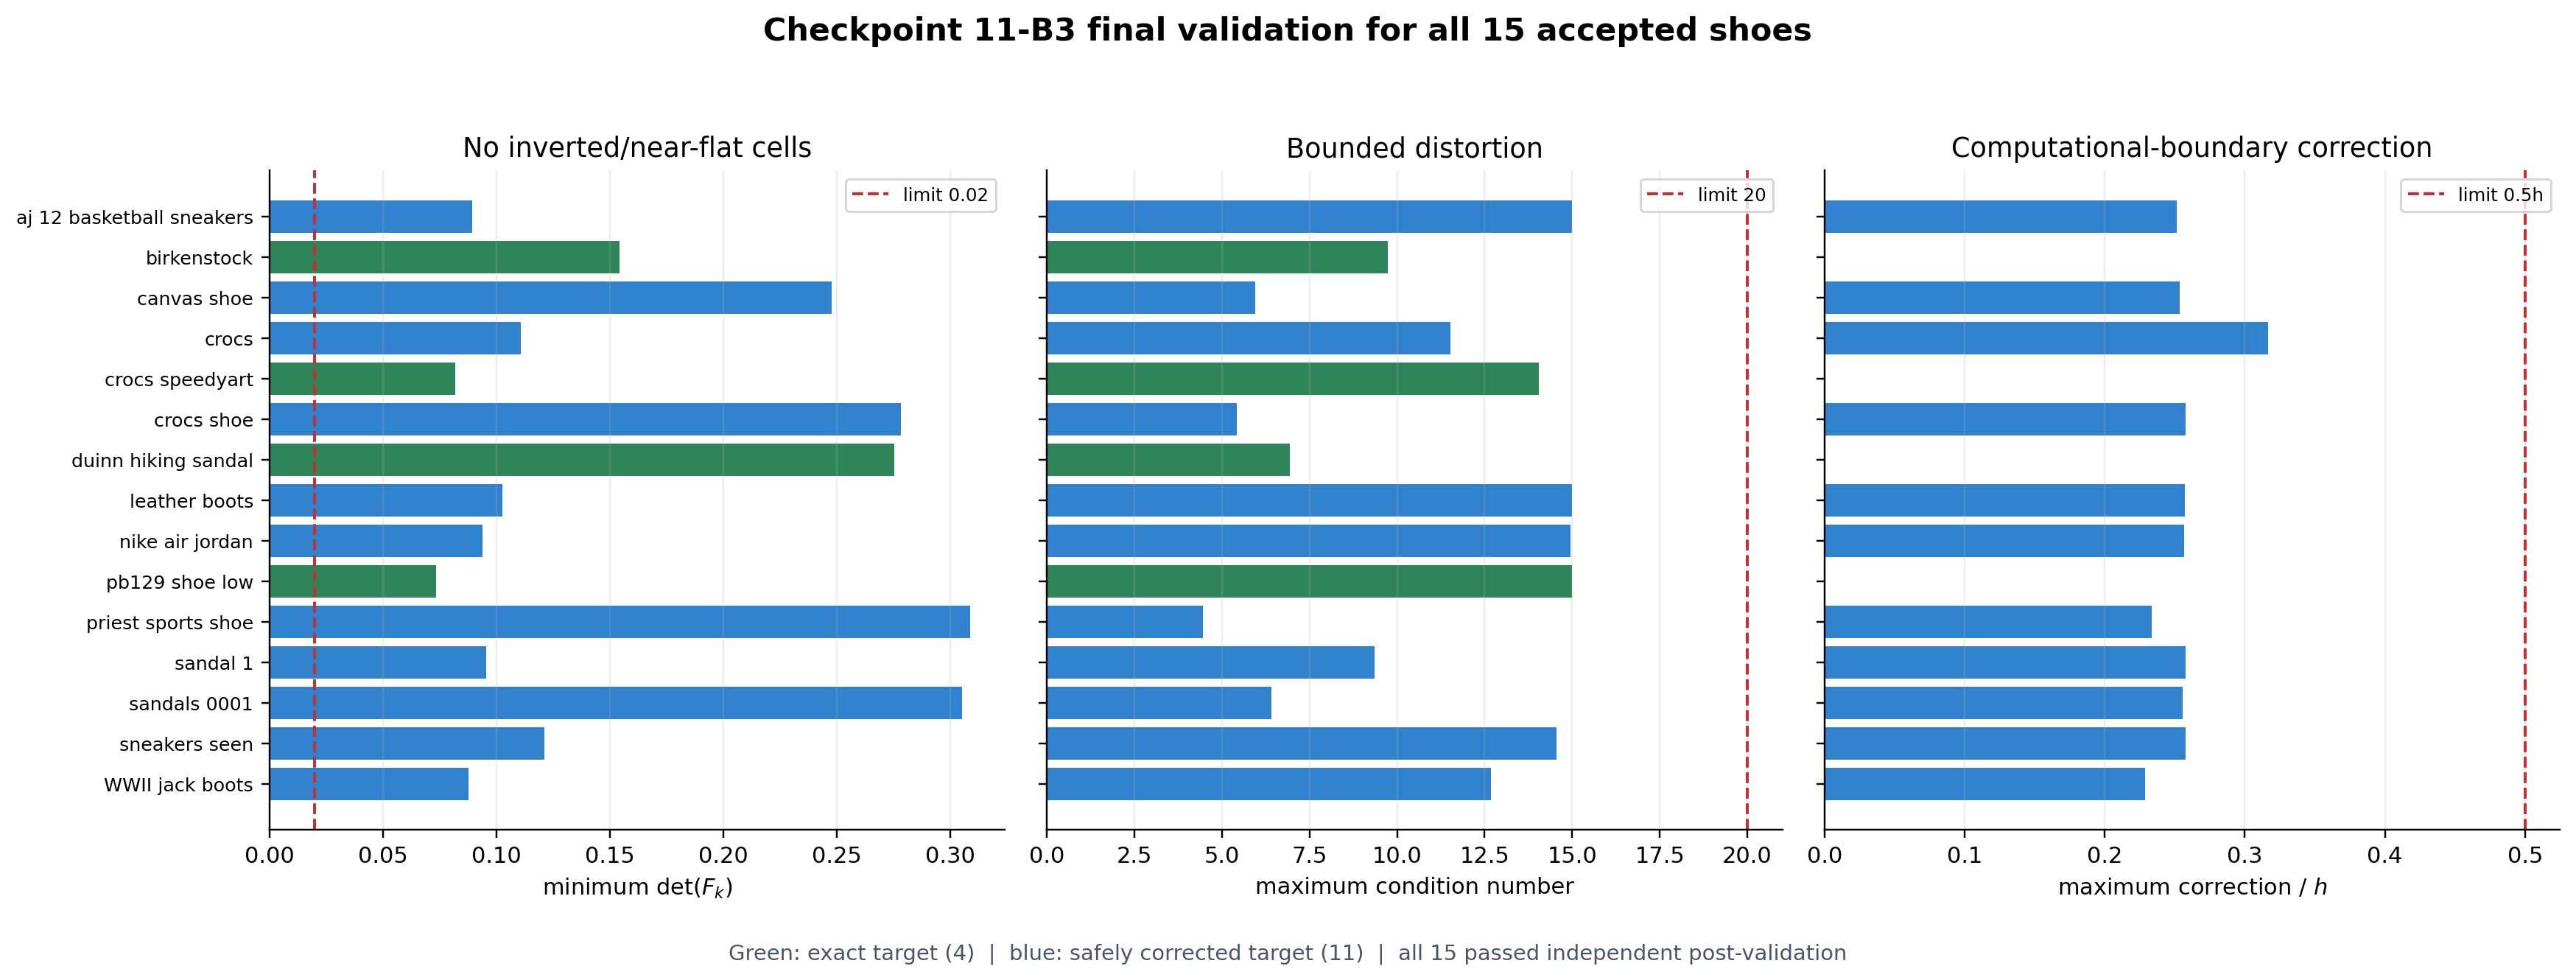
\includegraphics[width=\textwidth]{08_batch_validation.png}
  \caption{Per-shoe final B3 metrics. The red dashed lines are fixed acceptance limits,
  not fitted per-shoe thresholds. Every bar remains on the accepted side.}
  \label{fig:b3-batch}
\end{figure}

For one cell, the singular values of $F_k$ give the local metric bounds

\begin{equation}
  \sigma_{\min}(F_k)\|dq\|_2
  \le \|dx\|_2
  \le \sigma_{\max}(F_k)\|dq\|_2.
\end{equation}

Thus the B3 singular-value and condition-number tests are the implemented local analogue
of the bounded-distortion requirement in Eq.~\eqref{eq:document-bounded-distortion}.
Positive determinants prevent local folds; exact boundary collision checks and 11-C
overlap audits address global ambiguity.

\section{Checkpoint 11-C: exact forward and inverse volume maps}
\label{sec:11c}

Checkpoint 11-C is a deterministic lookup layer over the completed B3 grids. It does not
deform, repair, optimize, or remesh anything.

For canonical tetrahedron $k$ with corners $Q_{k,0},\ldots,Q_{k,3}$, instance corners
$X_{i,k,0},\ldots,X_{i,k,3}$, and barycentric weights $\lambda$, the forward map is

\begin{equation}
  \chi_i(k,\lambda)=\sum_{a=0}^{3}\lambda_aX_{i,k,a}.
  \label{eq:forward-map}
\end{equation}

For inverse lookup of physical point $x$, define

\begin{equation}
  D_{X,k}=[X_{i,k,1}-X_{i,k,0}\quad
           X_{i,k,2}-X_{i,k,0}\quad
           X_{i,k,3}-X_{i,k,0}].
\end{equation}

For each conservative candidate tetrahedron,

\begin{equation}
  \begin{bmatrix}\lambda_1\\\lambda_2\\\lambda_3\end{bmatrix}
  =D_{X,k}^{-1}(x-X_{i,k,0}),
  \qquad
  \lambda_0=1-\lambda_1-\lambda_2-\lambda_3.
  \label{eq:inverse-barycentric}
\end{equation}

If all weights lie within the fixed tolerance, the canonical point and harmonic value are

\begin{align}
  \Phi_i(x)&=\sum_{a=0}^{3}\lambda_aQ_{k,a},\\
  r(x)&=\sum_{a=0}^{3}\lambda_a r_{k,a}.
  \label{eq:inverse-map}
\end{align}

The containing-tetrahedron search uses a conservative uniform AABB grid with 32 cells on
the longest axis. A tetrahedron spanning more than 512 cells enters a global conservative
list. Exact AABB and barycentric tests decide containment; there is no nearest-cell
snapping. If several adjacent tetrahedra contain a face/edge/vertex query and reconstruct
the same canonical point, the smallest ID is chosen deterministically. Disagreeing
canonical reconstructions are reported as \texttt{NONINJECTIVE\_OVERLAP}.

Finite points outside the tetrahedral shell are classified using the final triangulated
boundaries as inside computational anatomy, outside the envelope, or numerically
ambiguous. The knee truncation remains mappable but is excluded from footwear-support
queries. Non-finite rows receive an independent status. The API accepts posed-SUPR,
normalized-shoe, and original-shoe frames; lookup itself always occurs in posed-SUPR
coordinates using the verified containment-fit transforms.

\begin{figure}[H]
  \centering
  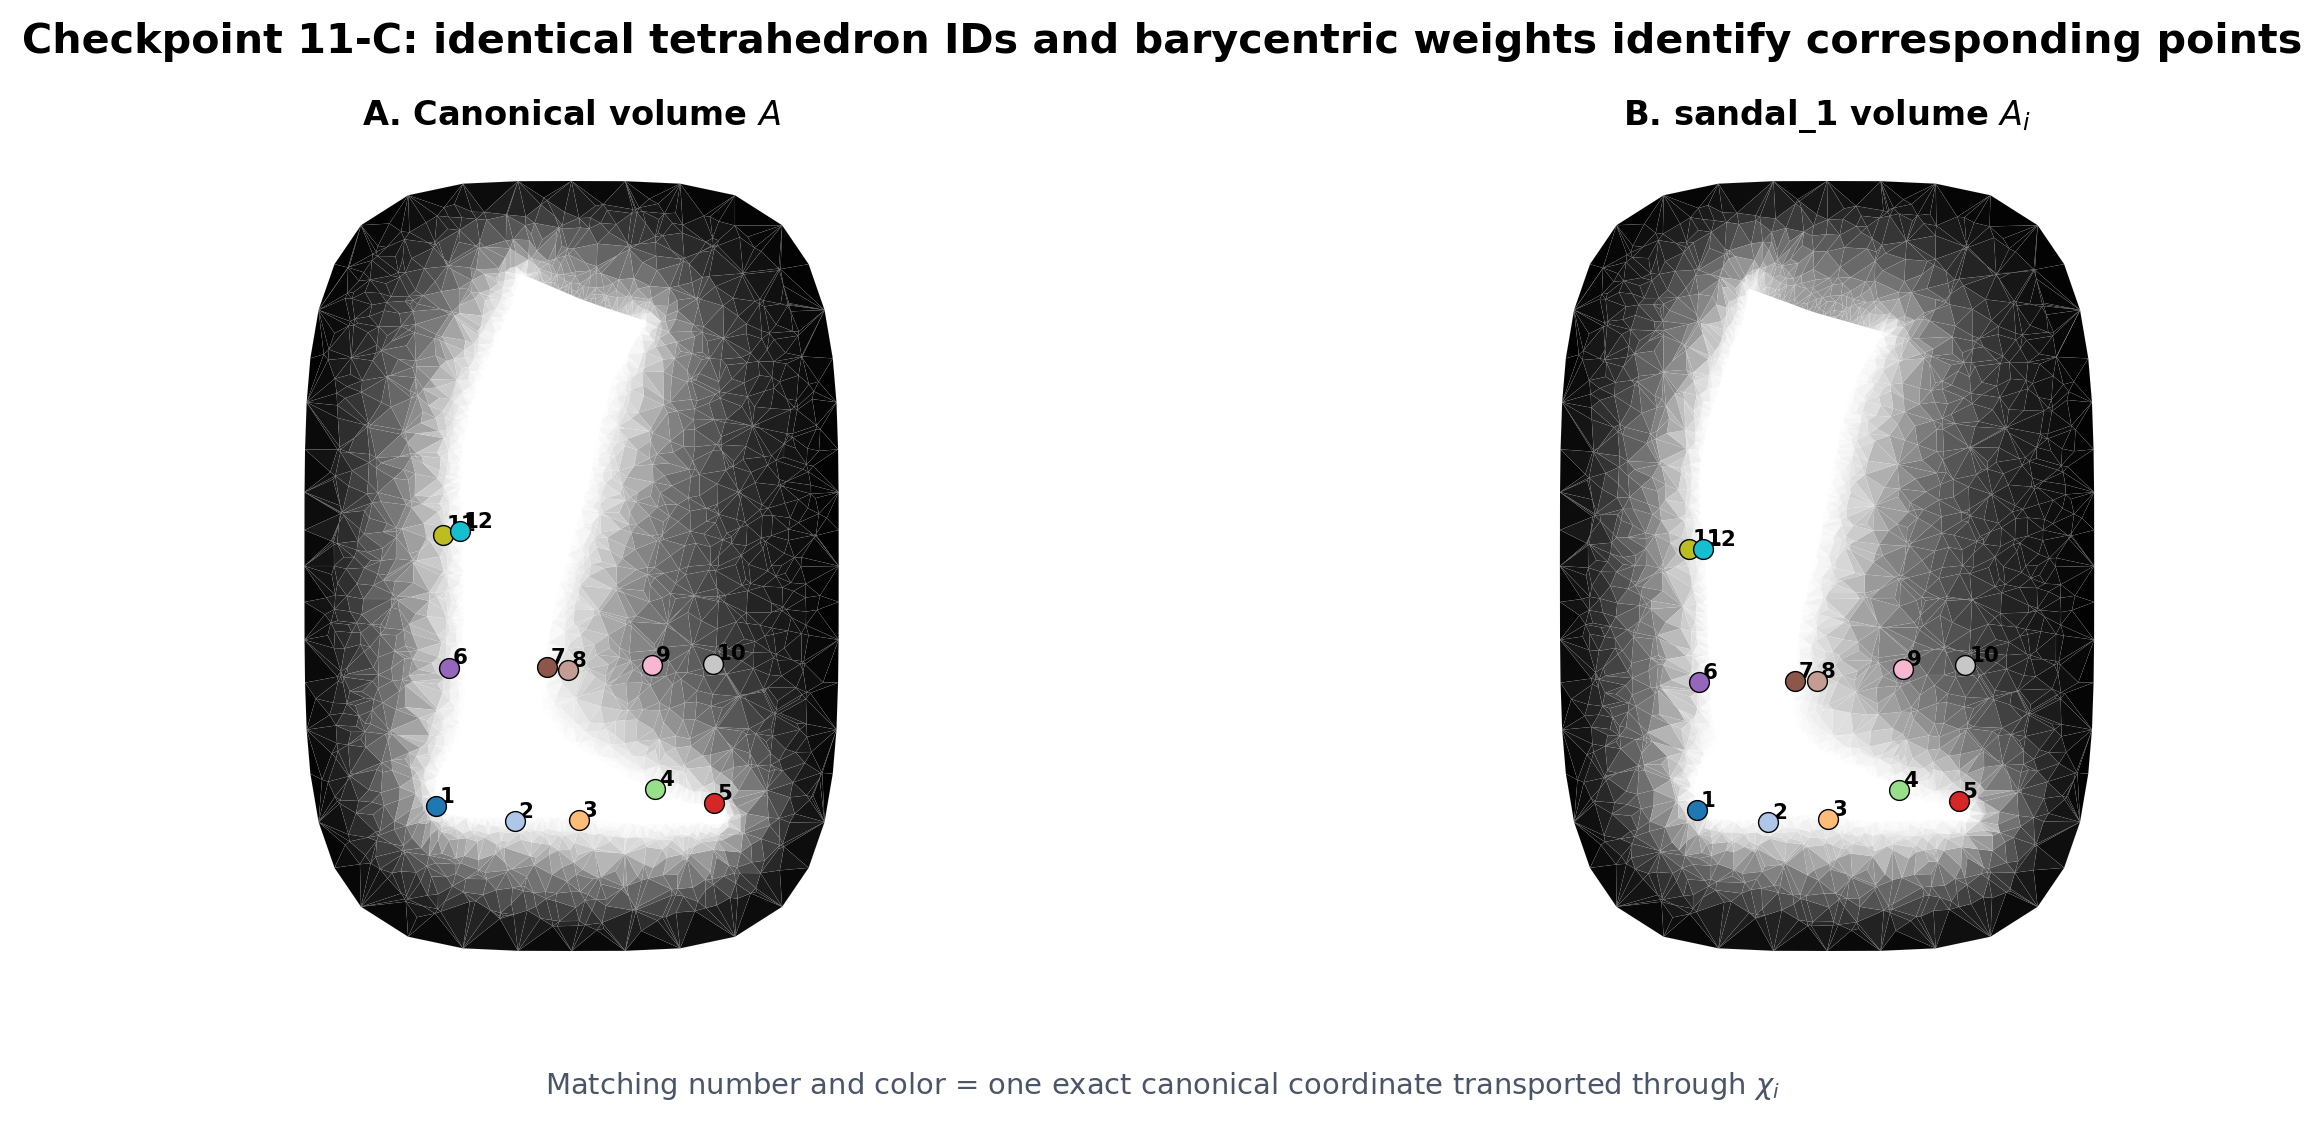
\includegraphics[width=\textwidth]{07_exact_mapping.png}
  \caption{Representative exact coordinates transported from canonical volume $A$ to
  the final \texttt{sandal\_1} volume. Each matching label uses the same tetrahedron ID
  and barycentric weights; its Euclidean position changes while its canonical identity
  remains fixed.}
  \label{fig:mapping}
\end{figure}

\subsection{Exhaustive deterministic audit}

For every accepted shoe, 11-C queried five strictly interior weight patterns in every
one of the 59,081 tetrahedra:

\begin{equation}
  (0.25,0.25,0.25,0.25),\quad
  (0.55,0.15,0.15,0.15),\quad \text{and its three permutations}.
\end{equation}

This gives 295,405 strict interior queries per shoe. The audit also checked all 14,440
volume vertices, all 127,024 unique tetrahedral face centroids, 15,584 anatomical-boundary
face centroids, 860 knee-cap face centroids, 1,280 outer-boundary face centroids, and 256
samples in each external coordinate frame.

All 15 shoes report \texttt{mapping\_valid}. No noninjective overlap was found. Every
generated valid-domain sample was mappable and all forward/inverse, physical, canonical,
harmonic-$r$, shared-boundary, and frame round trips passed. For \texttt{sandal\_1}, the
maximum strict-interior canonical round-trip error was $1.113\times10^{-15}$ and maximum
physical error was $7.027\times10^{-16}$ in normalized computational units.

The required identities are therefore observed numerically:

\begin{equation}
  q\xrightarrow{\chi_i}x\xrightarrow{\Phi_i}q'\approx q,
  \qquad
  x\xrightarrow{\Phi_i}q\xrightarrow{\chi_i}x'\approx x.
\end{equation}

\section{Where the project is in \texttt{representation.pdf}}

\begin{figure}[H]
  \centering
  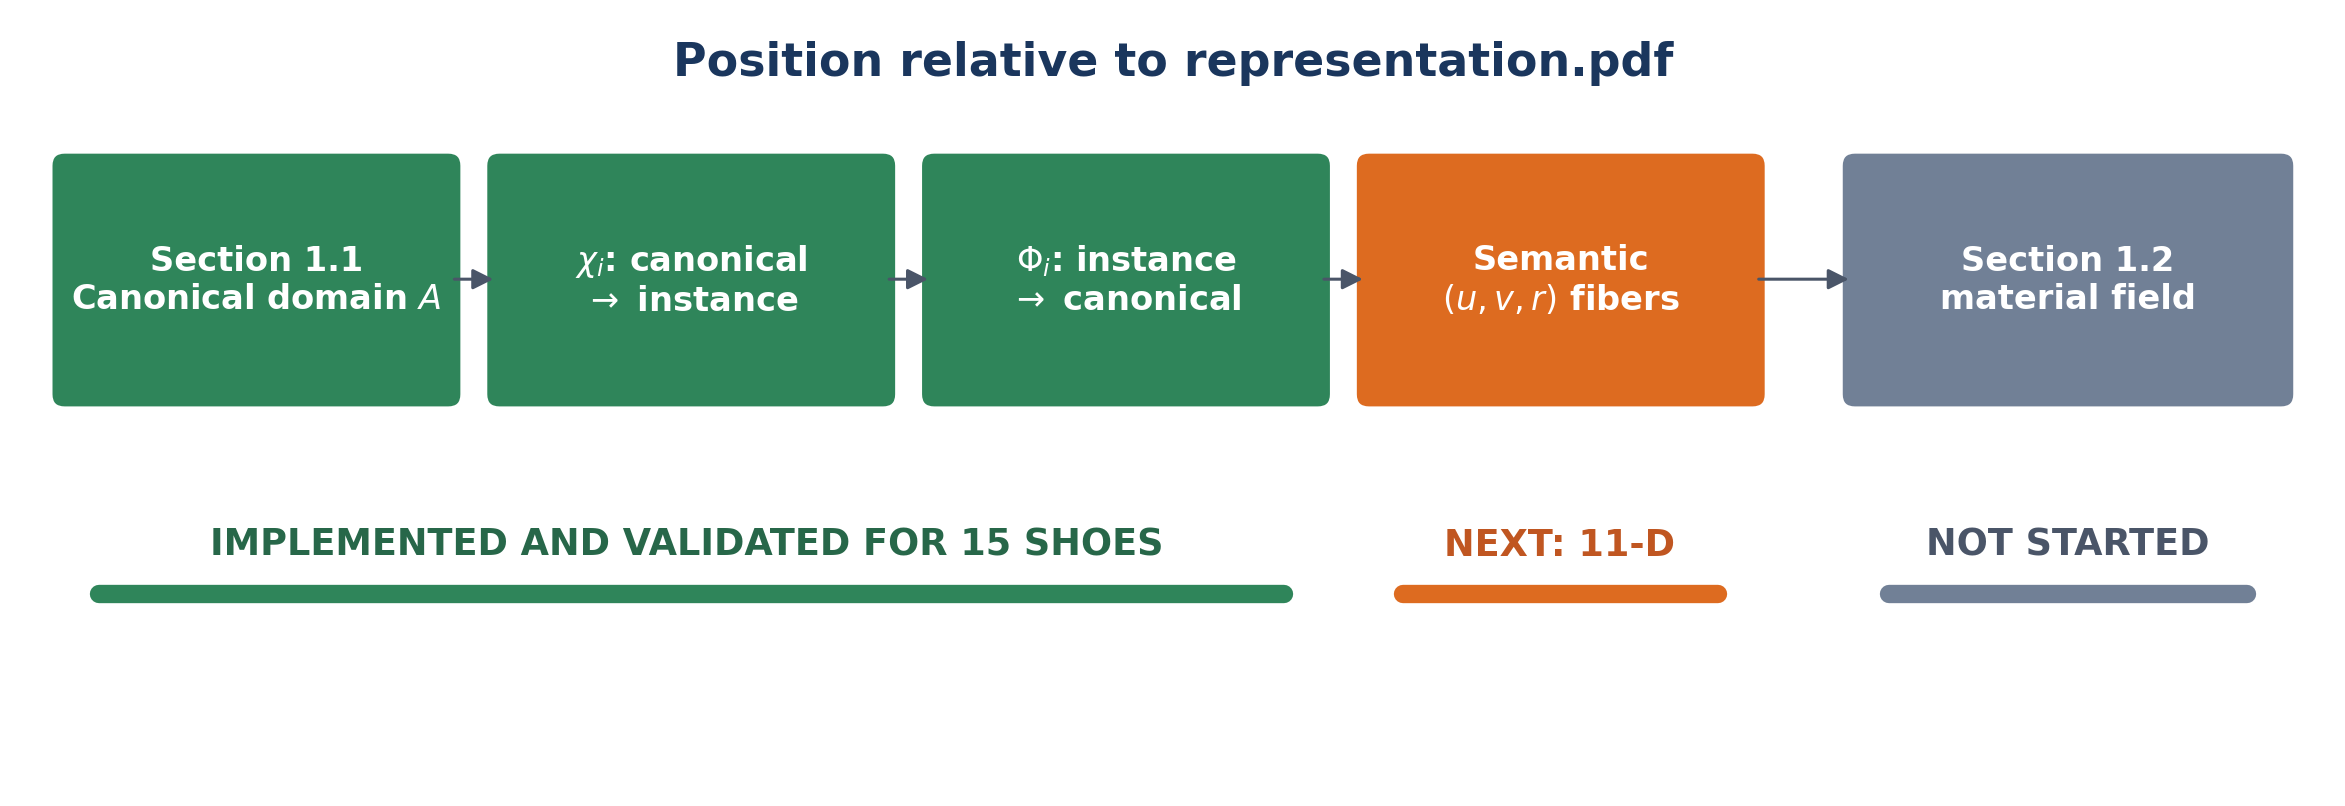
\includegraphics[width=\textwidth]{09_document_progress.png}
  \caption{Current boundary between completed and pending work.}
  \label{fig:document-progress}
\end{figure}

\subsection{Section 1.1: what is complete}

The following geometric substrate is implemented for 15 shoes:

\begin{itemize}
  \item a canonical foot-and-lower-leg domain $A$;
  \item one valid fitted volume $A_i=N(F_i)$ per accepted shoe;
  \item shared tetrahedron IDs and connectivity;
  \item positive, bounded-distortion piecewise-affine deformations;
  \item exact forward $\chi_i$ and inverse $\Phi_i$ queries;
  \item transported harmonic $r$;
  \item explicit rejection/classification outside the mathematical domain.
\end{itemize}

This establishes the exact computational realization of the map proposed in
Eq.~\eqref{eq:document-map}. It also provides the shared location system required before
learning any footwear prior.

\subsection{Checkpoint 11-D: what remains in Section 1.1}

The exact internal address in Eq.~\eqref{eq:exact-coordinate} is not yet the document's
semantic notation $(u,v,r)$. The harmonic scalar $r$ exists, but a volume point has not
yet been assigned a unique anatomical surface origin $(u,v)$. Checkpoint 11-D must build
and validate canonical anatomical fibers

\begin{equation}
  \gamma_{u,v}(r)\subset A,
  \qquad
  \gamma^i_{u,v}(r)=\chi_i(\gamma_{u,v}(r)),
\end{equation}

that start on anatomical skin, move monotonically outward, stay inside the valid domain,
do not fold/reverse, reach the envelope as intended, and never terminate on the
computational knee cap. A single flattened global UV map is not required: canonical
surface face ID plus three barycentric weights can serve as the exact $(u,v)$ chart.

\subsection{Section 1.2 and beyond}

Section 1.2 has not started. After 11-D, shoe triangles or material samples can be mapped
through $\Phi_i$ and aggregated in shared anatomical coordinates. The proposed fields are

\begin{equation}
  g_i(u,v),\qquad \delta_i^{\mathrm{in}}(u,v),\qquad
  \delta_i^{\mathrm{out}}(u,v),
\end{equation}

with base material field

\begin{equation}
  B_i(u,v,r)=\max\{g_i(u,v),
  \delta_i^{\mathrm{in}}(u,v)-r,
  r-\delta_i^{\mathrm{out}}(u,v)\}.
\end{equation}

Learning the anatomy-conditioned clearance prior, residual material field, signed
implicit footwear function, set-valued surface correspondence, and appearance/completion
model belongs to Sections 1.2--1.4 and is outside the current implementation.

\section{Conclusions and immediate next step}

The main result is not merely that 15 meshes were processed. The result is that 15 shoes
with different surface topology are now connected to one common anatomical volume while
preserving their individual fitted anatomy and shoe coordinate transforms. The final
volumes have fixed canonical connectivity, no folded cells, no surface intersections,
bounded distortion, and reversible point lookup.

The correct next step is Checkpoint 11-D: construct one canonical, validated semantic
fiber system and transport it to every instance through the already validated $\chi_i$.
Only after that should Section 1.2 convert footwear geometry into anatomical coverage and
inner/outer material extents. No learning is required or appropriate before this shared
semantic coordinate is complete.

\appendix
\section{Per-shoe B3 and 11-C summary}

\small
\begin{longtable}{@{}p{0.34\textwidth}p{0.13\textwidth}rrrr@{}}
\caption{Final geometry and mapping metrics. Correction is normalized by fitted surface
resolution $h$. All rows have zero final intersections and 11-C status
\texttt{mapping\_valid}.}\label{tab:per-shoe}\\
\toprule
\textbf{Shoe} & \textbf{B3 result} & $\min J$ & $\max\kappa$ & $\max\Delta/h$ & \textbf{11-C max. err.}\\
\midrule
\endfirsthead
\toprule
\textbf{Shoe} & \textbf{B3 result} & $\min J$ & $\max\kappa$ & $\max\Delta/h$ & \textbf{11-C max. err.}\\
\midrule
\endhead
AJ-12 basketball sneakers & corrected & 0.0895 & 15.00 & 0.252 & $1.58\!\times\!10^{-15}$\\
Birkenstock Arizona sandal & exact & 0.1545 & 9.74 & 0.000 & $9.93\!\times\!10^{-16}$\\
Canvas shoe & corrected & 0.2479 & 5.94 & 0.254 & $9.49\!\times\!10^{-16}$\\
Crocs & corrected & 0.1110 & 11.52 & 0.317 & $9.02\!\times\!10^{-16}$\\
Crocs (SpeedyArt) & exact & 0.0820 & 14.04 & 0.000 & $9.17\!\times\!10^{-16}$\\
Crocs shoe & corrected & 0.2783 & 5.43 & 0.258 & $9.16\!\times\!10^{-16}$\\
Duinn hiking sandal & exact & 0.2753 & 6.94 & 0.000 & $9.16\!\times\!10^{-16}$\\
Leather boots & corrected & 0.1027 & 15.00 & 0.257 & $1.86\!\times\!10^{-15}$\\
Nike Air Jordan & corrected & 0.0940 & 14.95 & 0.257 & $1.16\!\times\!10^{-15}$\\
PB129 low shoe & exact & 0.0735 & 15.00 & 0.000 & $1.98\!\times\!10^{-15}$\\
Priest sports shoe & corrected & 0.3087 & 4.45 & 0.234 & $9.17\!\times\!10^{-16}$\\
Sandal 1 & corrected & 0.0957 & 9.36 & 0.258 & $1.11\!\times\!10^{-15}$\\
Sandals 0001 & corrected & 0.3053 & 6.40 & 0.255 & $1.11\!\times\!10^{-15}$\\
Sneakers Seen & corrected & 0.1213 & 14.54 & 0.258 & $9.17\!\times\!10^{-16}$\\
WWII German jack boots & corrected & 0.0878 & 12.69 & 0.229 & $1.30\!\times\!10^{-15}$\\
\bottomrule
\end{longtable}
\normalsize

\section{Principal artifact locations}

\begin{description}[style=nextline,leftmargin=0pt]
\item[Previously reported support fits]
\footnotesize\nolinkurl{/home/ab5298/Outputs/FootShellGaussian/golden_set_evaluation/support_fit}\normalsize
\item[Cavity diagnoses]
\footnotesize\nolinkurl{/home/ab5298/Outputs/FootShellGaussian/golden_set_evaluation/cavity_analysis}\normalsize
\item[Containment-fitted anatomy]
\footnotesize\nolinkurl{/home/ab5298/Outputs/FootShellGaussian/golden_set_evaluation/containment_fit}\normalsize
\item[Dense and extended anatomy]
\footnotesize\nolinkurl{/home/ab5298/Outputs/FootShellGaussian/golden_set_evaluation/anatomical_surface}\newline
\footnotesize\nolinkurl{/home/ab5298/Outputs/FootShellGaussian/golden_set_evaluation/extended_anatomical_surface}\normalsize
\item[Canonical volume and 11-A targets]
\footnotesize\nolinkurl{/home/ab5298/Outputs/FootShellGaussian/golden_set_evaluation/anatomical_volume}\normalsize
\item[Accepted 15-shoe B3 batch]
\footnotesize\nolinkurl{/home/ab5298/Outputs/FootShellGaussian/golden_set_evaluation/instance_anatomical_volume/batch_threads1_20260913_181358}\normalsize
\item[Accepted 15-shoe 11-C audit]
\footnotesize\nolinkurl{/home/ab5298/Outputs/FootShellGaussian/golden_set_evaluation/instance_volume_mapping/batch_threads1_20260913_181358}\normalsize
\item[Representation design document]
\footnotesize\nolinkurl{/storage/Abhinay/Shell_Gaussian/notes/representation.pdf}\normalsize
\end{description}

\section{Reproducibility note}

The numerical statements in this report were read from the saved JSON/NPZ artifacts and
the implemented fixed configurations. The figures were rendered directly from the saved
PLY/NPZ meshes and fields using
\texttt{notes/shared\_anatomical\_volume\_report\_assets/generate\_figures.py}.
The B3 batch manifest records the exact source digests and one-thread numerical-library
policy used for the accepted run. No B3 or mapping artifact was modified while preparing
this report.

\end{document}
